% main.tex — ICML 2026 Mechanistic Interpretability Workshop submission.
% Self-contained two-column format (icml2026.sty not available in template cache;
% formatting approximates ICML long-format guidance). Tectonic-compiled.

\documentclass[10pt,twocolumn,letterpaper]{article}

\usepackage[letterpaper,margin=0.75in]{geometry}
\usepackage{amsmath,amssymb,amsfonts}
\usepackage{graphicx}
\usepackage{booktabs}
\usepackage{microtype}
\usepackage[hidelinks]{hyperref}
\usepackage{xcolor}
\usepackage{caption}
\usepackage{subcaption}
\usepackage{enumitem}
\usepackage{titlesec}
\usepackage[round,authoryear]{natbib}

\graphicspath{{figures/}{../code/figures/}}

\captionsetup{font=small,labelfont=bf,skip=4pt}
\titlespacing*{\section}{0pt}{1.4ex plus 0.4ex minus 0.2ex}{0.8ex plus 0.2ex}
\titlespacing*{\subsection}{0pt}{1.1ex plus 0.3ex minus 0.2ex}{0.6ex plus 0.1ex}

\setlength{\columnsep}{0.25in}
\setlength{\parskip}{2pt}

\title{\vspace{-1.0em}Where a VLM Fine-Tune Commits Depends on the Task:\\ Differential and Causal Localization in Nanonets-OCR2-3B}
\author{Mohammad Ali Shehral\\Northeastern University}
\date{}

\begin{document}

\makeatletter
\twocolumn[
\begin{@twocolumnfalse}
\maketitle
\begin{abstract}
\noindent
Nanonets-OCR2-3B is the largest public-weight checkpoint in a family whose flagship (Nanonets-OCR-3, 35B MoE) tops the IDP Leaderboard. Because OCR2-3B shares a public base --- Qwen2.5-VL-3B-Instruct --- it is a clean object for a question the flagship cannot answer: where does an OCR fine-tune actually commit? We apply four complementary diagnostics to 26 document images: residual-stream L2 diffs, head-level attention-pattern diffs, residual-stream activation patching, and per-module weight diffs. The residual signal concentrates in the upper decoder and peaks at L35 with Pearson $r = 0.996$ between two independently-trained fine-tunes of the same base. Per-image activation patching gives a sharper result than our pilot on 4 docvqa images implied: the causal-threshold layer is \emph{bimodal}. Eleven of 26 images flip at layers 0--2 --- all four arXiv-equation pages, handwriting, and non-Latin scripts. Fifteen of 26 flip at layers 9--15 --- English typewritten documents, forms, receipts, and one Chinese page. Median threshold $L = 10$. Under a corrected reference (Nanonets-OCR2-3B's shipped config mis-sets top-level \texttt{tie\_word\_embeddings}; we use the intended tied projection), the full residual-stream patch is genuinely OCR-directional: 26 of 26 images eventually produce OCR2's corrected top-1 at some layer, with a peak match rate of 92.3\% at L34 and a median first-match layer of 16. A random-matched-magnitude residual control produces 3.85\% peak match (1/26 images, 2 of that image's 36 layer-trials), a 24$\times$ differential that rules out a generic perturbation-tolerance reading. The fine-tune's causal commitment enters at input layers for content the base Qwen2.5-VL reads poorly, and at mid-decoder for content the base already reads. The router head L11.H14 from \citet{hua2025conflicting} ranks 141 of 576 in our attention-pattern diff. A head-level causal test shows that no single-head L11 patch and no full-L11 attention patch redirects base toward OCR2's top-1: patched predictions never match OCR2. What the head-level test does show is a destabilization gradient --- H14 destabilizes 3/26 images, a low-Frobenius L11 control (H7) destabilizes 2/26, the highest-Frobenius L11 head (H8) destabilizes 1/26, and the full-layer swap destabilizes 1/26. The three H14-destabilized images are 2/4 arXiv and 1/4 handwritten. The mid-decoder residual-level threshold must therefore involve L11 MLP and cross-layer dynamics, not L11 attention alone. Within the top-12 Frobenius-diff heads, the L0 cluster loses structured-marker attention (input re-encoding) and the L30--33 cluster gains it (output specialization). MLPs carry 69\% of the weight change; rank-16 SVD of the per-module diff recovers 39--67\% depending on the module, so a rank-16 LoRA on \texttt{mlp.gate\_proj} and \texttt{mlp.up\_proj} captures the largest share under a compact rank budget but is not a full-fidelity reproduction. The L35 residual peak is text-dominated (53\% pre-image instruction tokens, 27\% post-image, 20\% image tokens). OCR2's vision encoder is perturbed $1.60\times$ more than its decoder in fractional Frobenius terms (11.2\% vs.\ 7.0\% mean), but the parallel measurement on OCR-s gives 1.1\% --- an order of magnitude lower. The ViT edit is specific to how Nanonets trained OCR2, not a property of OCR fine-tuning the shared base.
\end{abstract}
\vspace{1em}
\end{@twocolumnfalse}
]
\makeatother

\section{Introduction}
\label{sec:intro}

The Nanonets OCR family's current flagship, Nanonets-OCR-3, tops the IDP Leaderboard at 85.9 overall, ahead of GPT-5.4 and Gemini-3-Pro. Its weights are not public --- OCR-3 is a 35B Mixture-of-Experts architecture released 2026-04-09 and available only through an API. The previous generation, Nanonets-OCR2-3B, is the largest public-weight member of the family: a Qwen2.5-VL-3B-Instruct \citep{qwenteam2025qwen25vl} fine-tune trained with the same structured-markdown SFT methodology as OCR-3. It reports 89.43 on DocVQA --- ahead of the 72B instruction-tuned Qwen2.5-VL base. We do not have the flagship's weights, but we have the public base and two independently-trained fine-tunes that share it. That is enough to ask a precise question: where in the model did the OCR fine-tune act?

The differential lens matters because most VLM interpretability studies a single trained model in isolation. \citet{hua2025conflicting} gave Qwen2.5-VL a clean head taxonomy under modality conflict: L11.H14 is a router, L19.H26 and L13.H26 are promoter heads.\footnote{L19.H26 and L13.H26 live in Qwen2.5-VL-7B's 28-head-per-layer layout; the 3B we analyze has 16 heads per layer, so those head indices do not exist in our model. We can only cross-check L11.H14.} \citet{steinberg2026ocrrouting} located OCR routing bottlenecks in three instruction-tuned VLMs. \citet{che2026counting} traced counting circuits in Qwen2.5-VL-7B. What none of these papers ask is the \emph{diff} question: when supervised fine-tuning turns a generalist VLM into an OCR specialist, what moves?

We ask it four times, with four methods. Residual-stream L2 diffs (\S\ref{sec:res-peak}) tell us where in the decoder the representational change accumulates. Attention-pattern Frobenius diffs (\S\ref{sec:attn}) tell us which heads see the world differently. Residual-stream activation patching (\S\ref{sec:causal}) tells us at which layer patching OCR2's state into the base is enough to flip the base's prediction --- this is the causal test the correlational diffs cannot do on their own. And a per-module weight diff (\S\ref{sec:weight}) tells us, in parameter space, what the fine-tune actually changed. The four measurements are internally consistent and suggest concrete next steps for a team adapting a similar VLM to a new document vertical.

Two findings are worth surfacing up front. First, the causal commitment does not happen at a single layer: it happens at different pipeline stages for different document types. Patching OCR2's residual into the base flips the top-1 at layers 0--2 for handwriting, LaTeX equations, and non-Latin scripts --- content the base reads poorly --- and at layers 9--15 for English typewritten documents, forms, and receipts --- content the base already reads. Across 26 images the threshold distribution is bimodal, median $L = 10$ and mode $L = 0$. Second, the fine-tune routes its weight change overwhelmingly through the MLP blocks --- \texttt{mlp.gate\_proj}, \texttt{mlp.up\_proj}, and \texttt{mlp.down\_proj} account for 69\% of the total Frobenius change. Together these sketch an allocation: for content near the base's existing territory, the payload lives in mid-decoder MLPs; for content far from it, the fine-tune also rewrites the input-side representation.

\section{Related Work}
\label{sec:related}

\paragraph{Cross-modal head taxonomy.} \citet{hua2025conflicting} identify three functional head types in Qwen2.5-VL under modality-conflict inputs: \emph{router} heads (modality-agnostic, follow the instruction), and \emph{image} / \emph{caption} promotion heads (always favor one stream). Their classification uses a 21-point $\alpha$-sweep; we treat their taxonomy as prior and look up one specific head (L11.H14) in our own attention-diff. Related: \citet{golovanevsky2024notice} characterize universal cross-attention heads in BLIP and LLaVA; \citet{baek2025ocrheads} identify ``OCR heads'' in Qwen2-VL-7B and InternVL2-8B via passkey / needle-in-a-haystack tests, finding that masking the top-20 OCR heads causes a $\sim$20\% DocVQA drop --- evidence that a small set of heads carry disproportionate OCR load in \emph{trained} models, orthogonal to our diff question.

\paragraph{OCR bottleneck localization.} \citet{steinberg2026ocrrouting} use causal PCA-subspace removal to locate OCR bottleneck layers in Qwen3-VL, Phi-4-multimodal, and InternVL3.5. They find architecture-specific bottlenecks (mid-depth for DeepStack models, earlier for single-stage projection). They study where OCR lives inside trained models; we study where fine-tuning \emph{moves representations}. The two measurements are complementary, and they are not in direct tension.

\paragraph{Circuit analysis of fine-tuning.} \citet{wang2025circuitlora} track circuits across fine-tuning of LLMs, finding that circuit nodes are stable while edges change 2--3$\times$ more, and that added nodes concentrate in middle and late layers. Their CircuitLoRA assigns LoRA rank proportional to edge-change magnitude. \citet{ma2025lorawhisper} dissect a LoRA-adapted Whisper encoder and find delayed specialization (early layers general, later layers task-specific). \citet{arditi2024refusal} show a safety fine-tune concentrates its behavioral effect in a single residual-stream direction. None of this has been done on a base-to-OCR-fine-tune pair.

\paragraph{Causal methods on VLMs.} \citet{li2025fcct} introduce FCCT, a three-pass (clean / corrupted / patched) causal tracing framework for VLMs that we borrow for \S\ref{sec:causal}. \citet{meng2022rome} established the template on GPT: mid-layer FFN modules carry factual associations, localizable by causal tracing. \citet{tigges2024circuitscale} show that circuit algorithms are stable across 70M--2.8B parameters across 300B training tokens even as specific head identities drift; this is the basis for transferring 3B findings upward.

\paragraph{Layer specialization.} \citet{neo2024visualinfo} show visual tokens become increasingly interpretable in vocabulary space as depth grows in LLaVA. \citet{skean2025layerbylayer} show intermediate layers can exceed final-layer quality on 32 downstream tasks, reminding us that a diff peak at the top of the stack is not the same as ``most information is there''.

\section{Method}
\label{sec:method}

\paragraph{Models.} All three models share the Qwen2.5-VL-3B-Instruct architecture: 36 decoder layers, 16 attention heads per layer (head dim 128), hidden size 2048, MLP intermediate size 11008, GQA with \texttt{num\_key\_value\_heads}=2, and a dynamic-resolution ViT vision tower. The models:

\begin{itemize}[leftmargin=1.4em,itemsep=0pt,topsep=0pt]
\item \textbf{base} --- \texttt{Qwen/Qwen2.5-VL-3B-Instruct}.
\item \textbf{OCR2} --- \texttt{nanonets/Nanonets-OCR2-3B}. Same base, structured-markdown SFT.
\item \textbf{OCR-s} --- \texttt{nanonets/Nanonets-OCR-s}. Earlier Nanonets fine-tune of the same base, used as a triangulation control for Claim 1.
\end{itemize}

Models are loaded sequentially on a consumer MPS device (Apple M4 Pro, 24 GB unified). Hooking uses \texttt{nnsight} v0.6.3 --- \texttt{transformer\_lens} does not register hook points inside VLM vision towers or image-token merge paths, so it is not applicable here.

\paragraph{Evaluation set.} 26 document images across 6 categories: printed mixed-layout (DocVQA, $n{=}6$), handwritten (IAM, $n{=}4$), scientific pages with LaTeX (arXiv crops, $n{=}4$), receipts (SROIE, $n{=}4$), forms (FUNSD, $n{=}4$), and multilingual (CH / AR / JA / FR, $n{=}4$). Each image is processed at $\sim$1000 patch-tokens via fixed \texttt{min\_pixels} / \texttt{max\_pixels} to keep activation tensor shapes consistent across runs.

\paragraph{Residual-stream L2 diff.} For image $x$, pair $(M_{\text{ft}}, M_{\text{base}})$, layer $L \in [0, 36]$:
\[
d_L(x, t) = \|\,h^{M_{\text{ft}}}_L(x, t) - h^{M_{\text{base}}}_L(x, t)\,\|_2.
\]
We aggregate over tokens $t$ (mean) and images $x$ (mean) to get a per-layer scalar. Two pairs are computed: OCR2 vs.\ base, OCR-s vs.\ base.

\paragraph{Head-wise attention-pattern diff.} For each decoder layer $L$, head $H$, image $x$:
\[
\delta_{L,H}(x) = \|\,A^{\text{OCR2}}_{L,H}(x) - A^{\text{base}}_{L,H}(x)\,\|_F.
\]
Aggregated over the 26 images. Total swept: $36 \times 16 = 576$ heads. We report the top-12 by mean $\delta$, and cross-reference L11.H14 explicitly because it is the prior-identified Qwen2.5-VL router head.

\paragraph{Marker-attention diagnostic.} For each head, we separately compute attention weight \emph{to} token positions of the structured markers in the prompt (\texttt{img}, \texttt{water}, \texttt{mark}, \texttt{page}, \texttt{\_number}, \texttt{signature}), averaged over the 26 images, and compare OCR2 vs.\ base. This is the direct test for ``this head specialized in marker emission'' --- a Frobenius-norm diff alone cannot distinguish input-encoding shifts from output-formatting shifts.

\paragraph{Residual-stream activation patching.} Following the three-pass structure of FCCT \citep{li2025fcct}, for each test image and each patching layer $L$: (i) run OCR2 forward, cache residual-stream activations at layer $L$; (ii) run base forward, replacing the layer-$L$ residual stream with OCR2's cached activations, then continuing the base forward from layer $L{+}1$ onwards; (iii) compare top-1 next-token prediction at the final generation position between the patched-base and the natural-base runs, and additionally record whether the patched base's top-1 matches OCR2's own last-token argmax. We also compute $\mathrm{KL}(\pi_{\text{patched}} \,\|\, \pi_{\text{natural-base}})$. Tested on all 26 evaluation images.

\paragraph{Corrected OCR2 reference.} Nanonets-OCR2-3B's \texttt{config.json} sets \texttt{tie\_word\_embeddings: False} at the top level while its \texttt{text\_config.tie\_word\_embeddings} is \texttt{True}, and the checkpoint ships no separate \texttt{lm\_head.weight}. HuggingFace's loader, reading only the top-level flag, initializes a random \texttt{lm\_head} (load report: ``\texttt{lm\_head.weight | MISSING | newly initialized}''), so OCR2's argmax via its own \texttt{lm\_head} is meaningless. Base's \texttt{tie\_word\_embeddings} is \texttt{True} correctly, so base's \texttt{lm\_head} is tied to \texttt{embed\_tokens.T} as intended. Base's \texttt{embed\_tokens} and \texttt{model.norm} weights are numerically identical to OCR2's (Frobenius fractional diff $0.000$ for both), so the \emph{corrected} OCR2 prediction for each image is \texttt{base.embed\_tokens.T} applied directly to OCR2's cached $h_{36}$ (the final cached hidden state, which is post-norm in HuggingFace's convention for this model --- verified by the characteristic RMS drop from $h_{35}$ to $h_{36}$). We use this as the reference for all match-OCR2 rates reported below. As a consistency check, applying \texttt{base.norm} to $h_{35}$ and then projecting yields the same corrected top-1 on 21 of 26 images; the five images where the two paths disagree (03 docvqa, 16 receipt, 19 form, 20 form, 24 multilingual\_ar) have close top-1 and top-2 logits under either path, consistent with argmax flips under bf16 precision.

\paragraph{Per-module weight diff.} Direct Frobenius-norm diff between OCR2 and base weights, per decoder layer, per module slot (\texttt{q\_proj}, \texttt{k\_proj}, \texttt{v\_proj}, \texttt{o\_proj}, \texttt{mlp.gate\_proj}, \texttt{mlp.up\_proj}, \texttt{mlp.down\_proj}). Also computes the fractional change (diff norm over base norm) per layer, and truncated-SVD rank recovery curves per module.

\paragraph{Modality-boundary probe (null).} We originally planned a logistic probe to distinguish structured-marker token positions from content-token positions. Because the Nanonets instruction prompt places structured markers at a fixed suffix, the probe reduced to position decoding and was abandoned. Pivoted to an image-token vs.\ text-token probe; both base and OCR2 hit 100\% at all 37 layers --- a ceiling-effect null. Documented here and listed as future work; no figure is included.

\paragraph{Vocabulary.} We use \emph{perturbed} and \emph{shifted} for correlational attention-pattern changes, reserving \emph{causal} for the patching results only. We call the 576-head diff leaders ``high-Frobenius heads'' --- we do \emph{not} relabel them as routers or promoters, because our method is not the $\alpha$-sweep that earns those labels in \citet{hua2025conflicting}.

\section{Results}
\label{sec:results}

\subsection{The residual-stream edit concentrates in the upper decoder, with a peak at L35}
\label{sec:res-peak}

\begin{figure}[t]
\centering
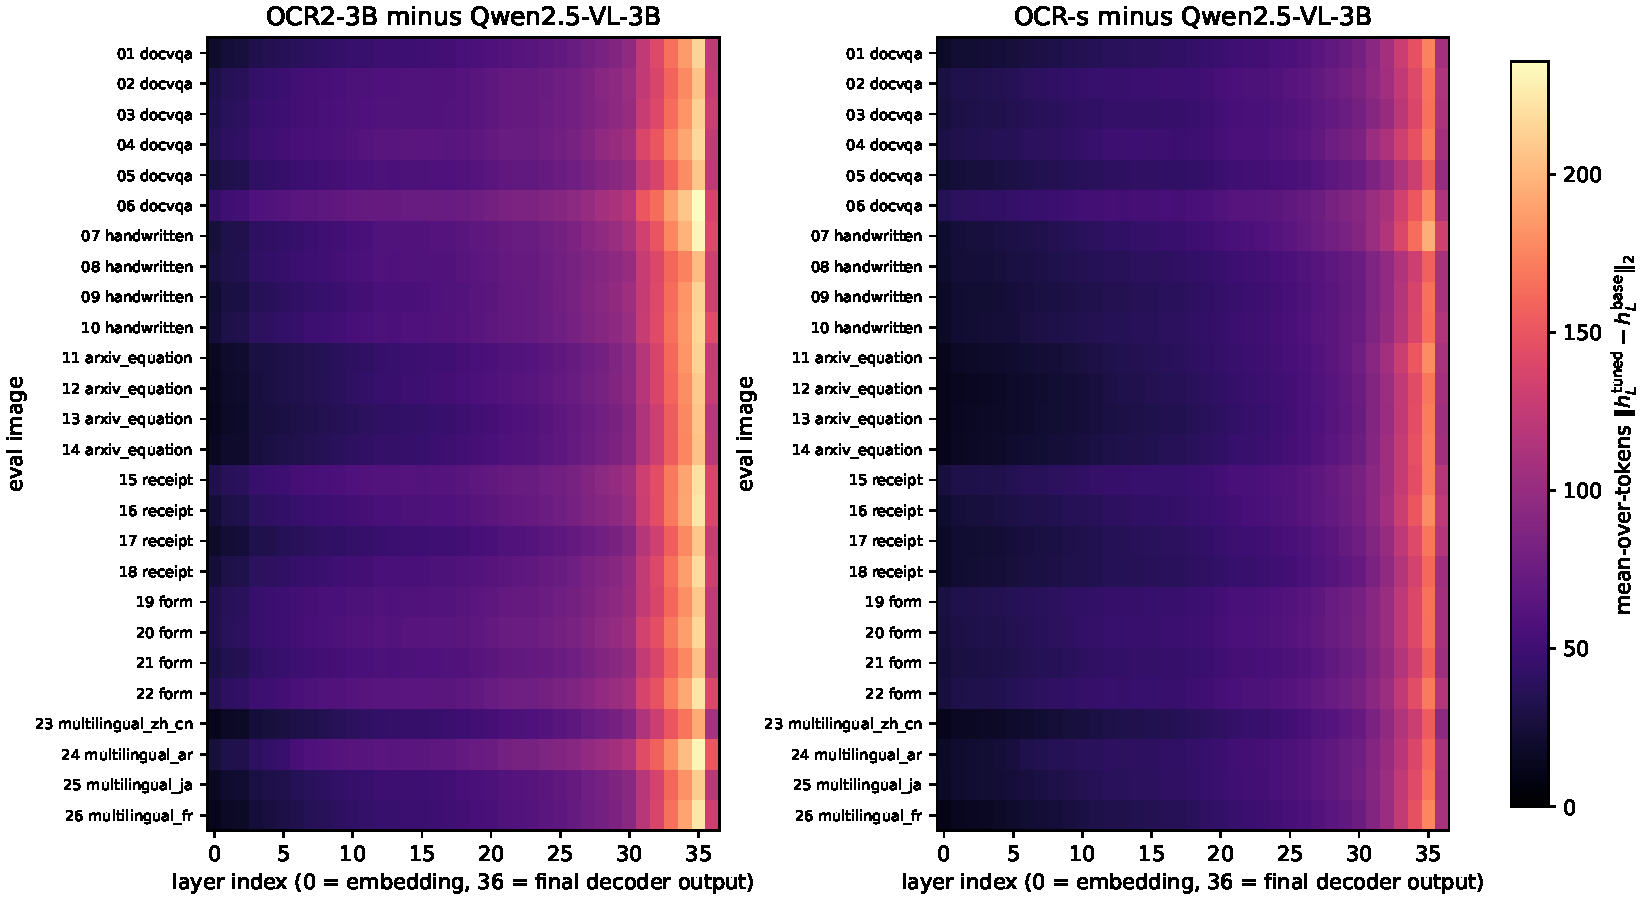
\includegraphics[width=\linewidth]{fig1_residual_diff.pdf}
\caption{Per-image, per-layer mean-over-tokens residual-stream L2 diff. Left: OCR2 vs.\ base. Right: OCR-s vs.\ base. Every row (26 images, 6 categories) lights up in the same L30--35 strip, and both fine-tunes share the same layer pattern. Image-averaged peaks: 214.4 (OCR2) and 168.8 (OCR-s), both at L35; cross-pair Pearson $r = 0.996$ on the 37-layer averaged curves. The drop at L36 is the post-norm projection.}
\label{fig:residual}
\end{figure}

Figure~\ref{fig:residual} shows the core Claim 1 result. OCR2 vs.\ base climbs from 25.0 at L0 through roughly 57 at L17, then ramps sharply through the upper decoder: 100.2 at L30, 214.4 at L35. The peak-to-floor ratio is 8.56$\times$. The last-four-layer mean (176.4) is 5.7$\times$ the first-four-layer mean (31.1). L36 is the post-norm projection and drops back to 129.3 --- expected, not a flaw.

The clincher is the second curve. OCR-s, trained separately on different data but from the same base, peaks at the same layer (L35, 168.83), and the entire 37-layer curve tracks OCR2's at Pearson $r = 0.996$. Two independently-trained fine-tunes agreeing on a 37-point curve at $r = 0.996$ is evidence that the concentration is a property of the base model's decoder geometry rather than of any single fine-tune's training data. The argument is correlational: it does not establish that either fine-tune's \emph{causal} commitment is at L35 (that is the question for \S\ref{sec:causal}). It also does not extend to the vision encoder. A parallel measurement in \S\ref{sec:vit} shows OCR2's and OCR-s's ViTs move at different magnitudes (11.2\% vs.\ 1.1\% mean fractional change) and correlate only at $r = 0.51$ across 32 blocks. Decoder-side reproducibility does not imply vision-side reproducibility.

Per-image variance is small: \emph{all 26} images individually peak at L35 --- zero variance in argmax. All 6 categories peak at L35 (Figure~\ref{fig:per-category}), with per-category peak values within 5\% of each other (208.70 for arXiv, 217.68 for receipts). The multilingual category does not inflate the average.

\begin{figure}[t]
\centering
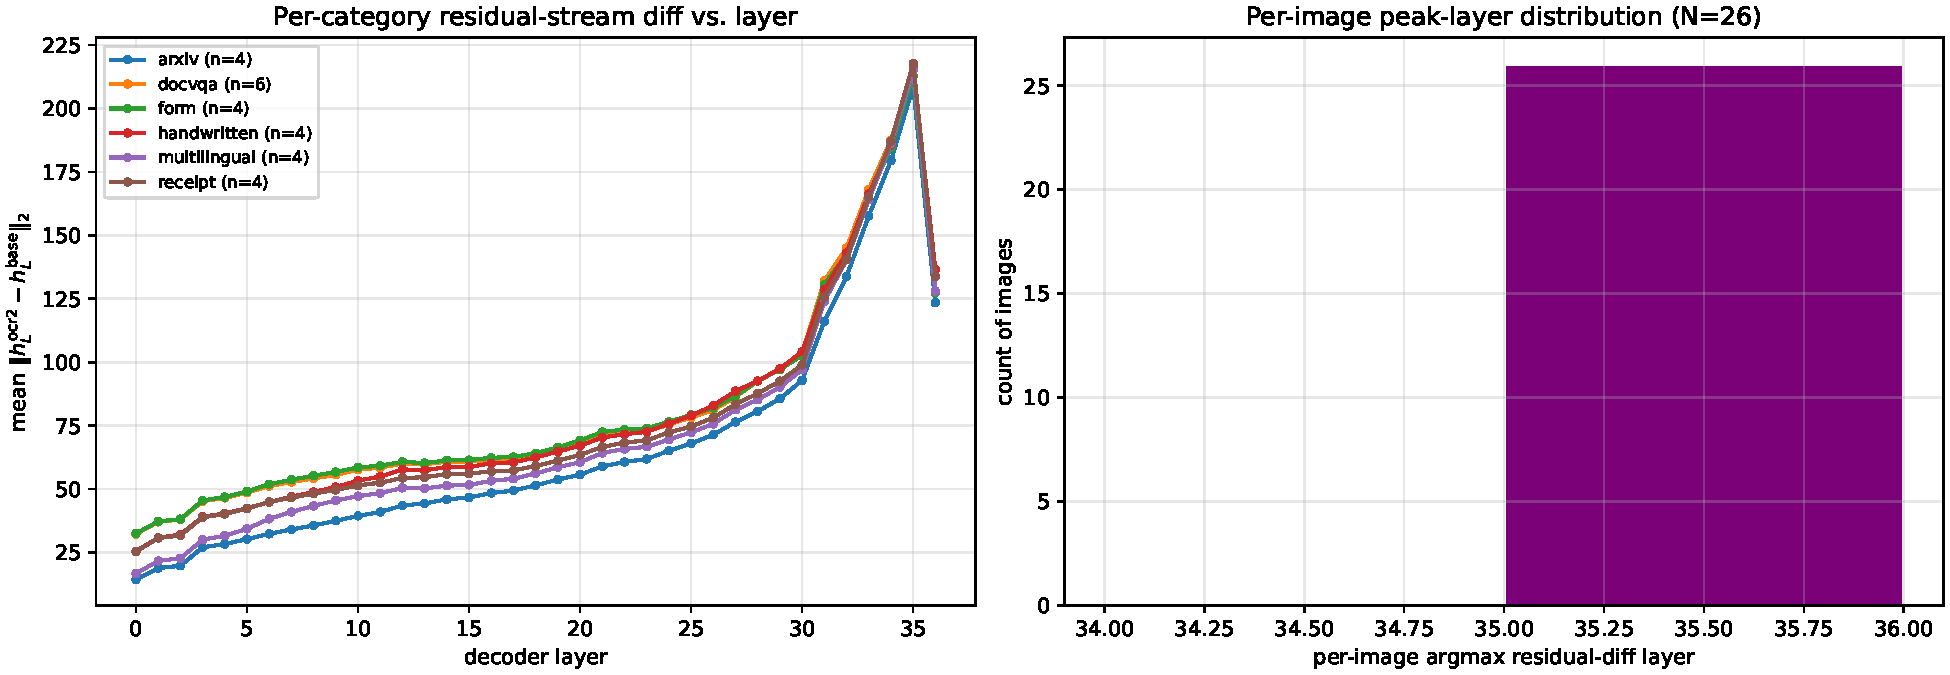
\includegraphics[width=\linewidth]{fig1b_per_category.pdf}
\caption{OCR2-vs-base residual diff broken out by document category. Every category peaks at L35 within 4\%. Multilingual sits in the middle of the spread.}
\label{fig:per-category}
\end{figure}

A careful reader will note that residual-stream L2 magnitude grows with depth in transformers regardless of fine-tuning. The 100$\rightarrow$214 jump over five layers, however, is sharper than baseline drift explains --- the prior 30 layers contribute only a 4$\times$ rise. We soften the language accordingly: \emph{concentrated in L30--35 with a peak at L35}, not \emph{localized to L35}.

Two decompositions of the L35 peak sharpen its interpretation. First, a per-block contribution diff --- the layer-$L$ output difference $(h_{L+1}-h_L)_{\text{OCR2}}-(h_{L+1}-h_L)_{\text{base}}$, rather than the cumulative state difference shown in Figure~\ref{fig:residual} --- concentrates at the last six decoder blocks: L30--L35 account for 46.3\% of total per-block contribution and the top-five contributing blocks are L35, L33, L34, L32, L30 in that order. Weights move nearly uniformly (\S\ref{sec:weight}); activations concentrate late. Second, a token-type decomposition of the L35 diff into pre-image instruction tokens, image-token positions, and post-image continuation tokens reveals a text-dominated peak: 53\% of the L35 L2 diff is carried by pre-image instruction tokens, 27\% by post-image text, and only 20\% by the image tokens themselves. The split is essentially category-invariant: all six document categories sit at 52--54\% pre, 19--22\% image, 25--28\% post, despite their causal thresholds from \S\ref{sec:causal} differing by up to 15 layers. The L35 signal is not an image-representation edit, and its token-type composition does not carry the bimodality of the causal-threshold result: the fine-tune reshapes prompt and output processing uniformly across content types, and the content-conditional story is a statement about \emph{where} (layer) the commitment is made, not \emph{how} it is distributed across tokens at the top of the stack.

\subsection{The causal threshold is bimodal, and depends on what the base already reads}
\label{sec:causal}

\begin{figure}[t]
\centering
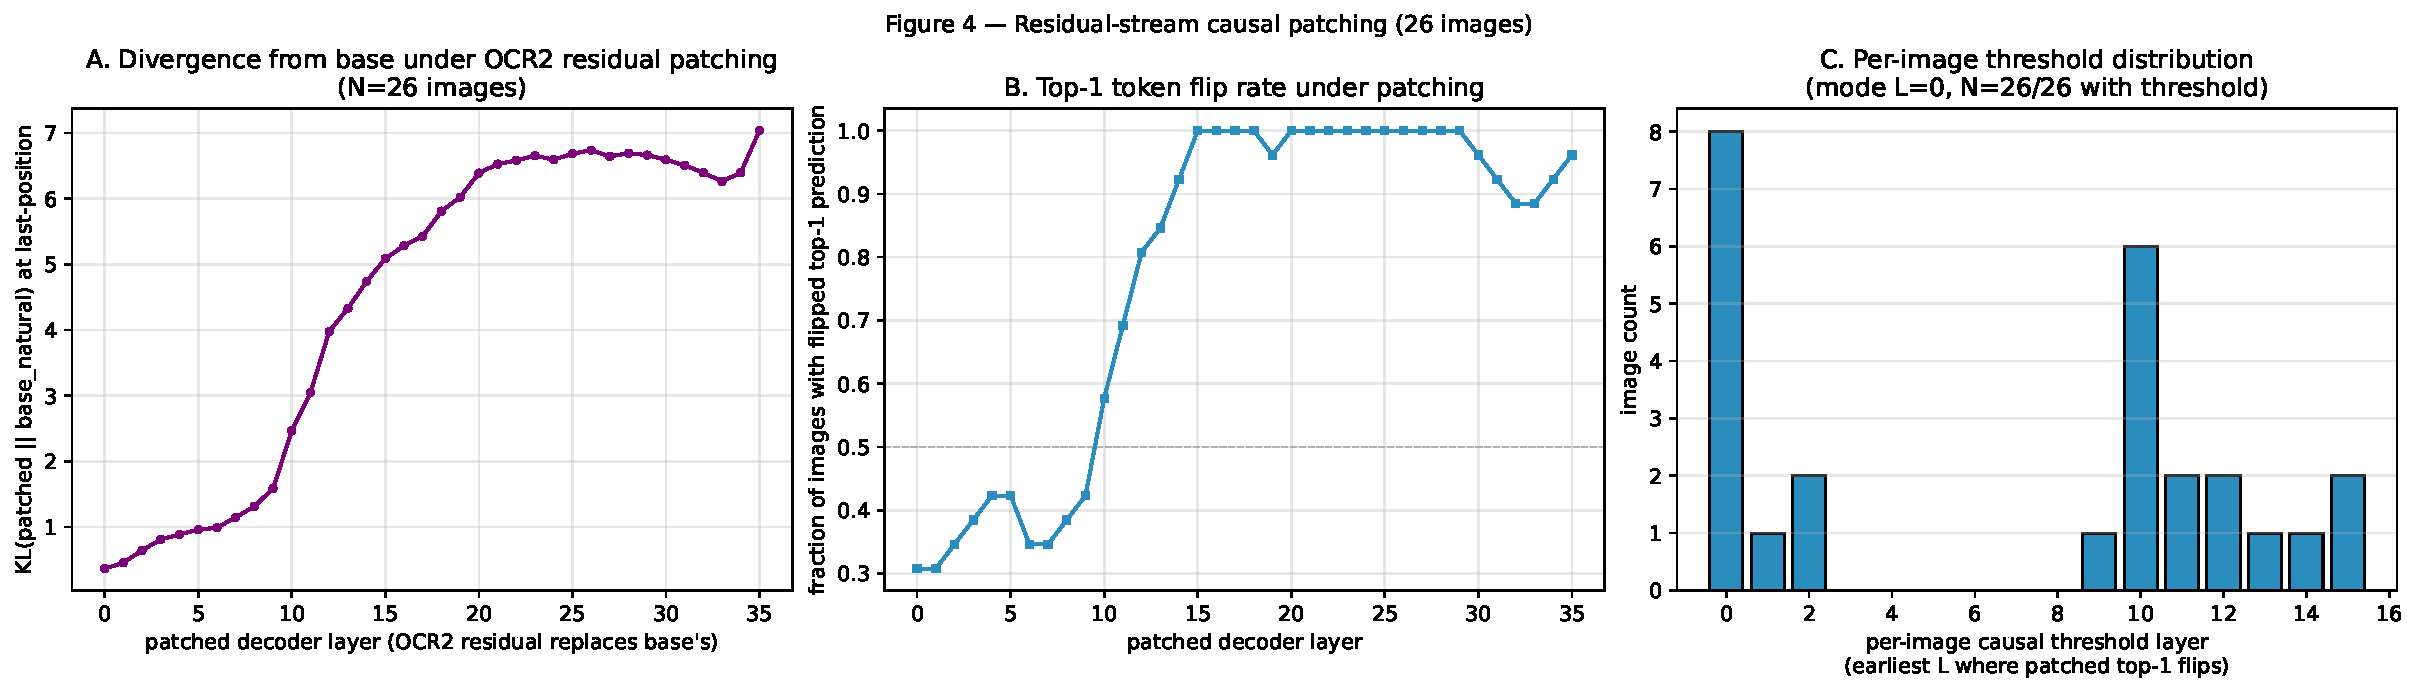
\includegraphics[width=\linewidth]{fig4_causal_patching.pdf}
\caption{Residual-stream activation patching, $N = 26$ images. At each layer $L$, we replace the base model's residual stream with OCR2's cached residual stream and let the base model finish the forward pass. Panel A: mean KL divergence from the unpatched base at the last-position distribution, by category. Panel B: per-image top-1 flip indicator ($1 =$ patched base matches OCR2's top-1) as a heatmap over layer $\times$ image. Panel C shows the distribution is bimodal, not a tight peak: 11 images have a threshold in layers 0--2 (arXiv equations, handwriting, non-Latin scripts) and 15 images in layers 9--15 (docvqa, forms, receipts, one Chinese page). Mode $L = 0$ (8 images), median $L = 10$, mean $L = 6.8$.}
\label{fig:patching}
\end{figure}

A pilot on 4 docvqa-heavy images suggested a clean step function at $L = 11$: every tested image flipped there, and no image flipped below L10. Re-running patching on the full 26-image evaluation set overturns the sharpness of that reading. The threshold layer --- the lowest $L$ at which the patched base's top-1 equals OCR2's top-1 --- is \emph{bimodal} across images, not modal. Figure~\ref{fig:patching} Panel C gives the full distribution.

The bimodality aligns with document content, not with noise. Of the 26 per-image thresholds, the early cluster (layers 0--2, 11 images) contains every arXiv-equation page (4/4, all threshold $L = 0$), all four handwritten pages ($[0, 2, 0, 2]$), and the three non-Latin multilingual pages (Arabic $L = 0$, Japanese $L = 1$, French $L = 0$). The middle cluster (layers 9--15, 15 images) contains the six docvqa pages ($[10, 10, 11, 12, 12, 15]$), all four FUNSD forms ($[10, 11, 13, 15]$), all four SROIE receipts ($[9, 10, 10, 10]$), and the one zh\_cn multilingual page ($L = 14$). The split is essentially: does the base Qwen2.5-VL already know how to read this, yes or no.

A reading consistent with this split is that the OCR fine-tune commits at two different pipeline stages depending on what the image demands. When the content is outside the base's reading repertoire --- handwriting, LaTeX equations, non-Latin scripts --- the fine-tune's work begins at the \emph{input}: patching OCR2's $h_0$ or $h_1$ into the base is already enough to flip the prediction, meaning the earliest residual-stream slots are where OCR2's reading of the image diverges enough from base's to change the final answer. When the content is within the base's repertoire --- English typewritten documents, receipts, forms --- the fine-tune's work begins in the \emph{mid-decoder}: patching at layers 9--15 is where the flip happens, consistent with the Qwen2.5-VL base reading the input fine and then being overridden by fine-tune-specific structured-output computation later in the stack.

This is a qualitatively different picture than the pilot suggested. The original $L = 11$ figure was an artifact of a docvqa-heavy sample; the full-26 reading is that there is no single causal threshold for the fine-tune. There are two, and which one applies is determined by whether the base already has a representation for the visual content.

Two caveats carry over. KL grows monotonically past each per-image threshold (mean peak at the final layers, not at the per-image threshold layer), so the flip is a top-1 boundary, not a full-distribution one. And the categorical split above has small per-category $n$ (4--6 images per category); with this data we can distinguish the two clusters but not, e.g., rank handwriting against LaTeX within the early cluster.

\begin{figure}[t]
\centering
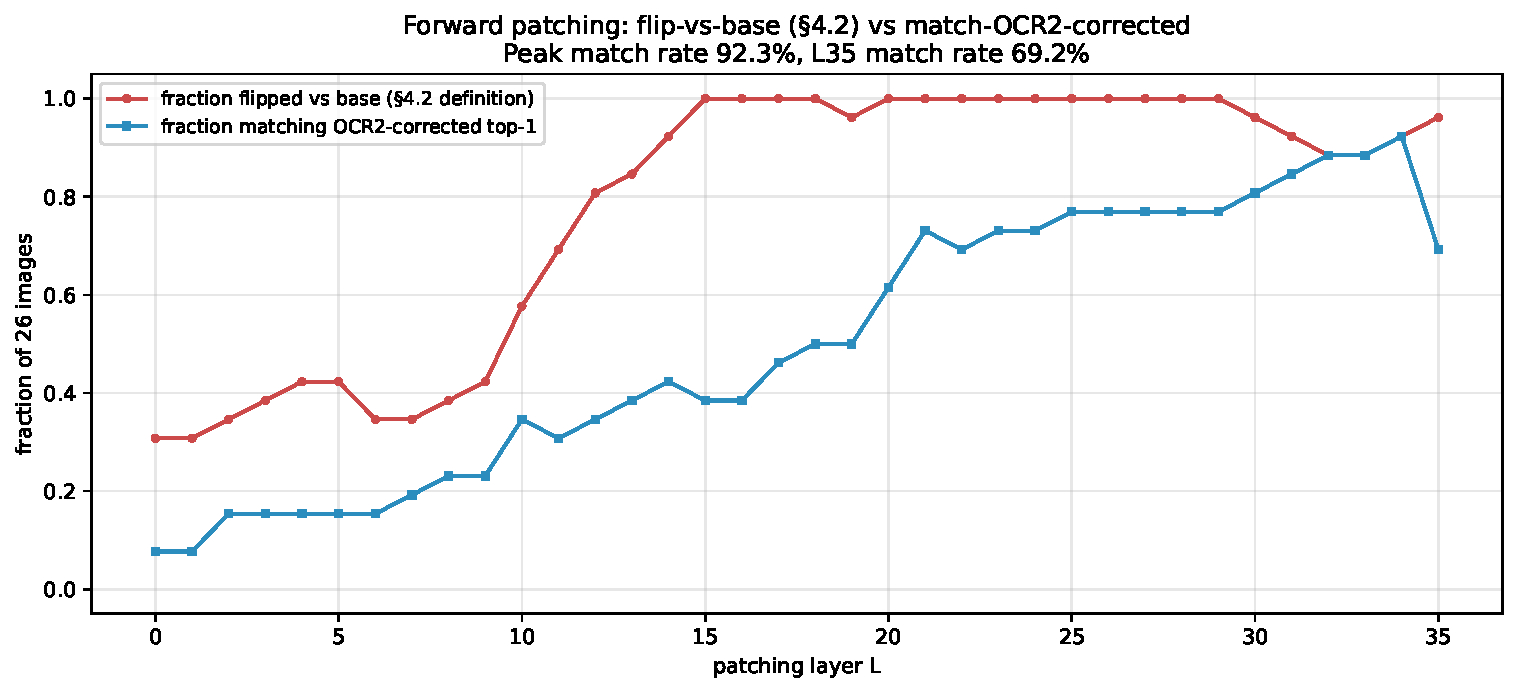
\includegraphics[width=\linewidth]{fig4c_match_corrected.pdf}
\caption{Forward patching under the corrected OCR2 reference (\S\ref{sec:method}). Red: fraction of images for which the patched base's top-1 differs from base's natural top-1 (the ``flip'' definition used in Figure~\ref{fig:patching}). Blue: fraction for which the patched base's top-1 \emph{matches OCR2's corrected top-1} --- i.e., the patched forward is OCR-directional, not merely destabilized. The blue curve rises to a peak of 92.3\% at L34 and drops to 69.2\% at L35 (the final-layer drop accounts for bf16 precision loss when the cached fp32 residual is cast to bf16 before the patch, combined with base's final-norm + lm\_head projection in bf16; L30--L34 values are 81\%, 85\%, 88\%, 88\%, 92\%). 26 of 26 images reach OCR2's corrected top-1 at \emph{some} layer; median first-match $L = 16$.}
\label{fig:fwd-match}
\end{figure}

The corrected-reference audit in Figure~\ref{fig:fwd-match} settles the question of what ``flip'' means in \S\ref{sec:causal}. The red curve (flip vs.\ base) rises to 100\% by L20 and reproduces the bimodal per-image threshold. The blue curve (match OCR2 corrected) rises more gradually --- 7.7\% at L0, 34.6\% at L10, 61.5\% at L20, 80.8\% at L30, 92.3\% at L34 --- and peaks at L34 immediately before base's final-norm + lm\_head projection. Twenty-six of 26 images eventually match OCR2's corrected top-1 at some layer, with median first-match $L = 16$. The flip and match curves have different shapes by construction: flip requires only that the patched base deviate from its own natural prediction, while match requires that the patched base converge on OCR2's specific prediction. Both signals are causal; the match curve is the stricter test, and the full residual-stream patch passes it for every image at a sufficiently deep layer.

This contrasts sharply with the head-level patching test in \S\ref{sec:head-patching}: full residual-stream patching redirects base toward OCR2's prediction for 26/26 images, but patching even all 16 heads at L11 redirects 0/26 (see also Figure~\ref{fig:head-patch}). The causal work at the mid-cluster residual threshold is carried by the full residual state at layer $L$, not by any L11 attention component alone; this is consistent with the 69\% MLP weight-share reported in \S\ref{sec:weight}.

The Hua et al.\ router layer observation survives but weakens. $L = 11$ is the layer of the documented cross-modal router head L11.H14, and in the 15-image middle cluster, 11 of 15 per-image thresholds sit at or above $L = 10$. We do \emph{not} claim the router head causes the flips --- head-level patching would be needed for that --- and the early-cluster images flip well before L11, so the router layer is not a universal threshold. The coincidence with Hua et al.\ is specific to the subset of documents the base already reads.

\subsection{L11.H14's attention pattern is stable, but its head-level causal role is not}
\label{sec:router-stable}

A complementary check against \citet{hua2025conflicting}: the attention pattern of the documented router head L11.H14 is not substantially perturbed by OCR fine-tuning. In our 576-head Frobenius sweep, L11.H14 has $\delta = 6.17$ and ranks 141 of 576 --- the 24.5th percentile from the top, with $z = +0.60$ relative to the 576-head global mean of 5.25. The top-12 have a floor of $\delta = 9.13$; L11.H14 does not enter the top quarter of the distribution.

A first reading of that number is that cross-modal arbitration is not where the fine-tune visibly acted, and we keep that reading for the attention-pattern statistic itself. But it is compatible with two different mechanistic stories: either the head is peripheral, or its routing function is preserved across fine-tuning while its output is used differently downstream. The attention-pattern diff cannot distinguish these --- we return to the distinction under direct causal intervention in \S\ref{sec:head-patching}, where the head turns out to be mechanistically load-bearing on a specific subset of content despite its stable attention.

\citet{hua2025conflicting} also identify two promoter heads, L19.H26 and L13.H26, but those indices refer to Qwen2.5-VL-7B's 28-head-per-layer layout. Our 3B base has 16 heads per layer; H26 is not addressable, and we restrict our cross-reference to L11.H14.

\subsection{Attention shifts split into L0 input re-encoding and L30+ marker specialization}
\label{sec:attn}

\begin{figure}[t]
\centering
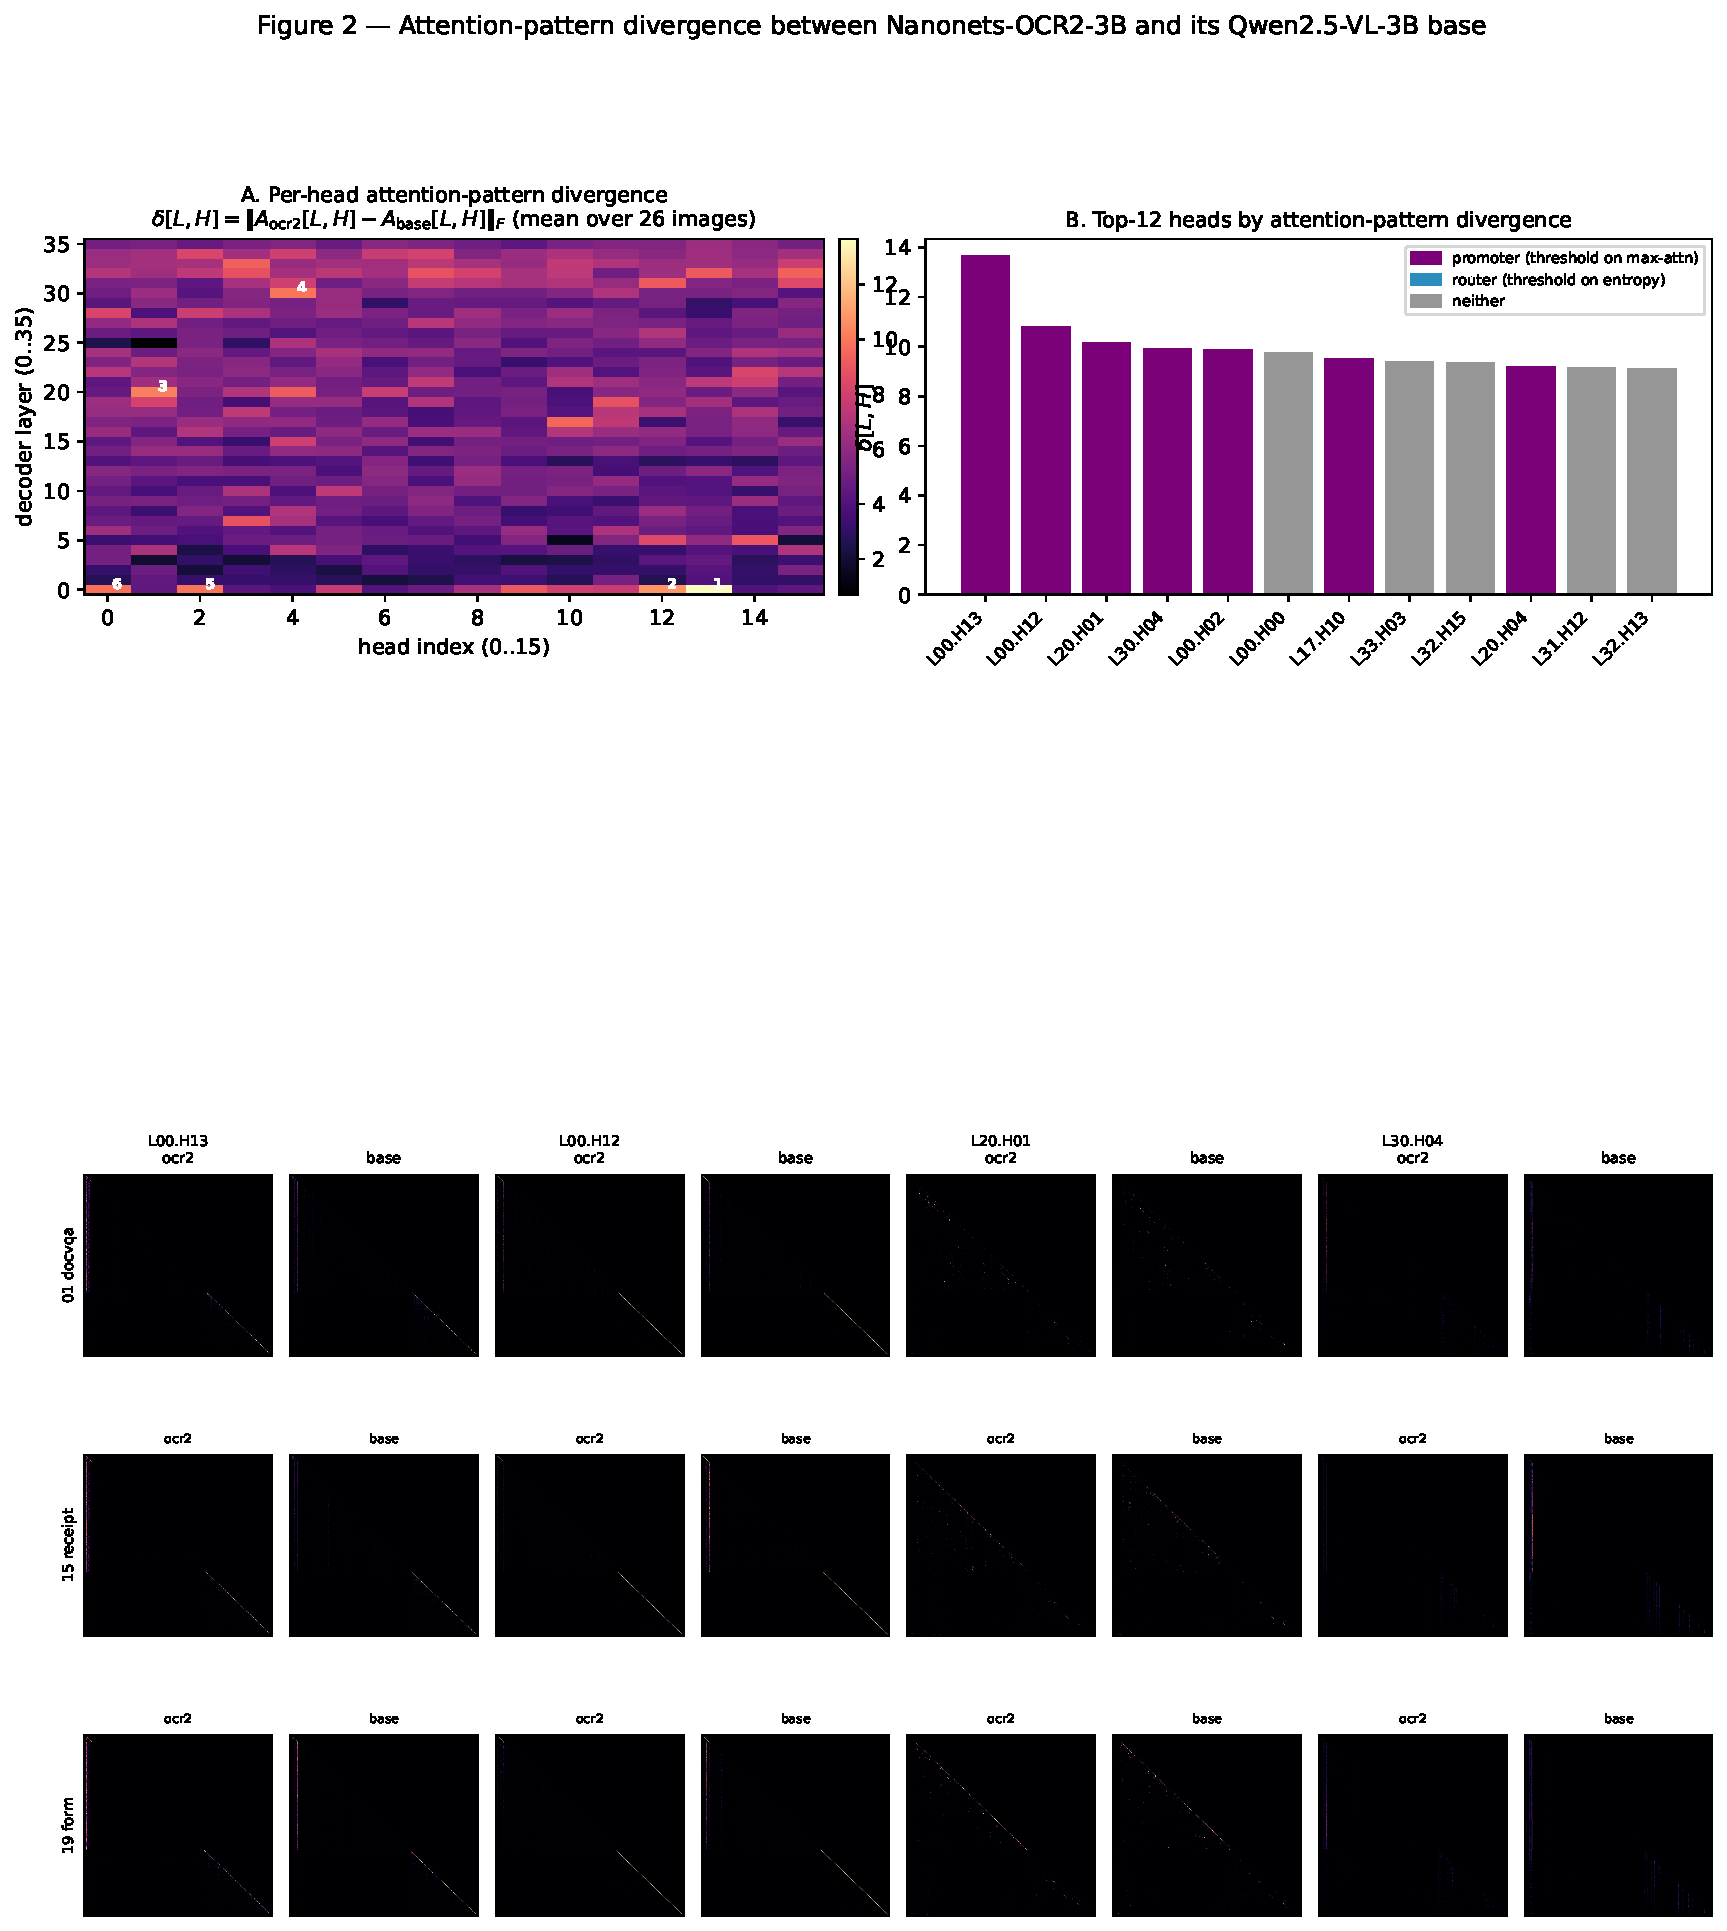
\includegraphics[width=\linewidth]{fig2_attention_diff.pdf}
\caption{Per-head attention-pattern Frobenius diff between OCR2 and base, swept over all 576 decoder heads. Top-12 heads span a bimodal layer distribution: 4 in L0--5 (early), 5 in L30--33 (late). The top head is L0.H13 at $\delta = 13.66$, $\sim 2.6\times$ the global-head mean. L11.H14 (the Hua et al.\ router head, green marker) is at rank 141 --- nowhere near the top tier.}
\label{fig:attn-diff}
\end{figure}

\begin{figure}[t]
\centering
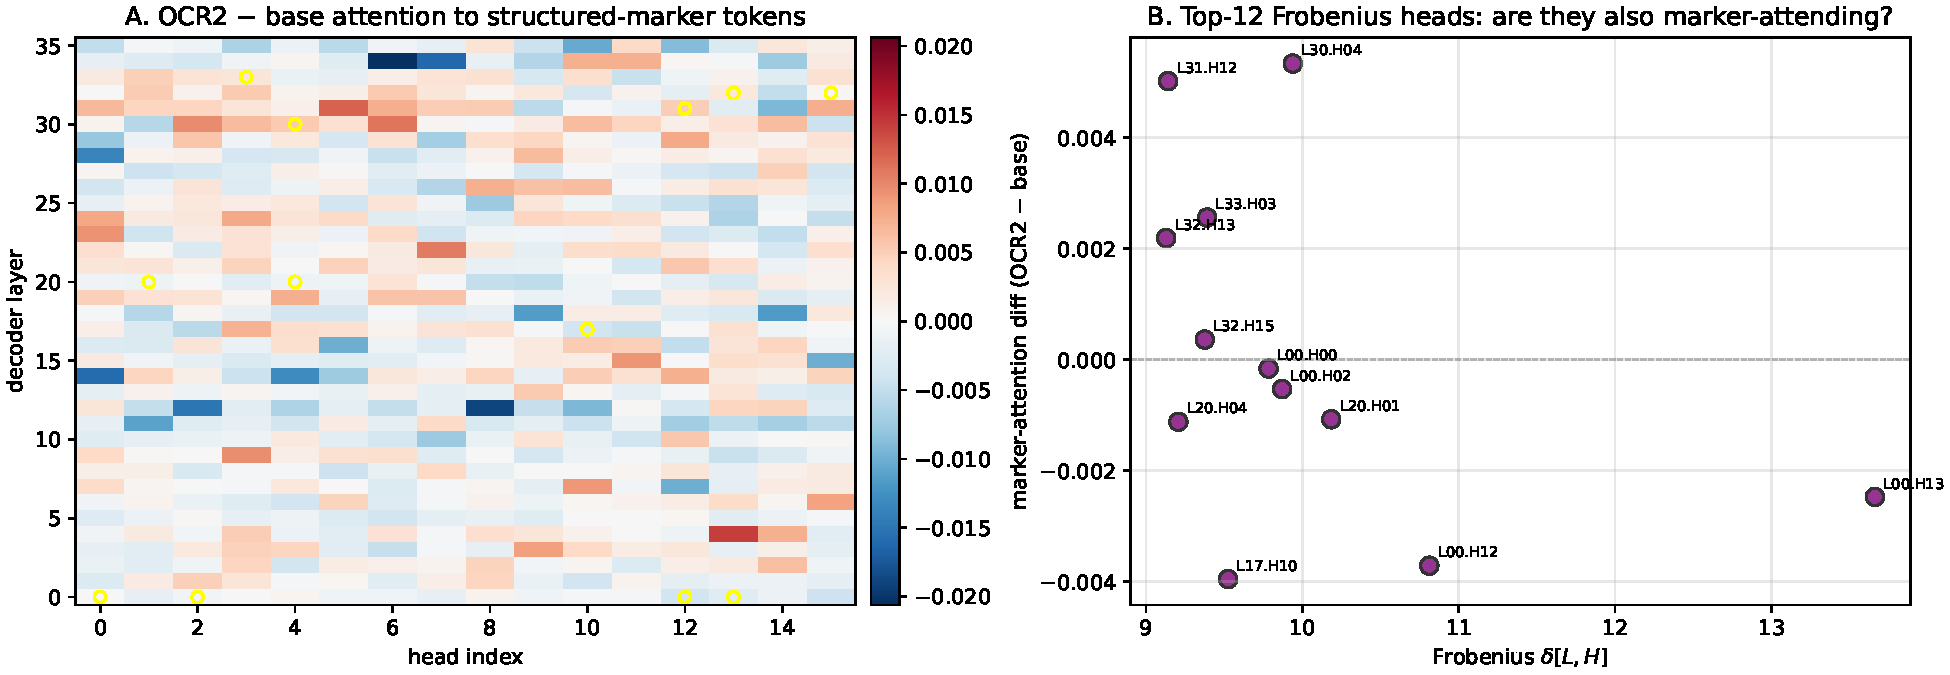
\includegraphics[width=\linewidth]{fig2b_marker_attention.pdf}
\caption{Attention weight to structured-marker token positions (\texttt{img}, \texttt{page}, \texttt{signature}, etc.) for the top-12 high-Frobenius heads, OCR2 minus base. The L0 heads 13, 12, 2, 0 \emph{decrease} marker attention under fine-tuning --- their behavior change is input re-encoding, not marker formatting. Heads L30.H04, L31.H12, L33.H03 \emph{increase} marker attention by $\sim 2\times$. Zero overlap between the top-12 Frobenius heads and the top-20 marker-attention gainers (L4.H13 is the single cleanest gainer, at +0.0143).}
\label{fig:marker-attn}
\end{figure}

\begin{figure}[t]
\centering
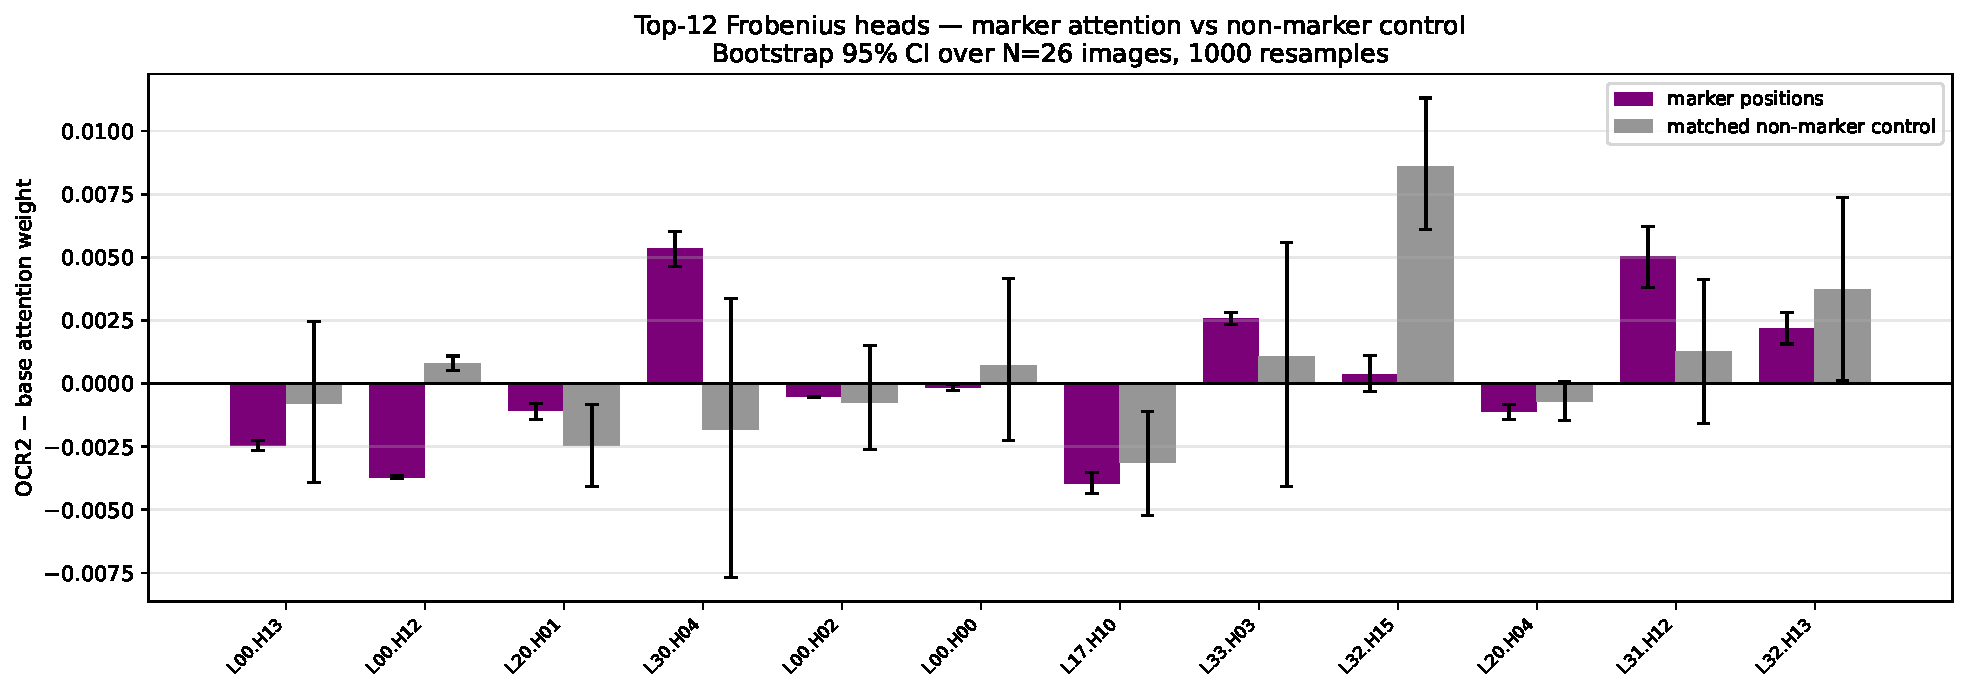
\includegraphics[width=\linewidth]{fig2c_marker_ci.pdf}
\caption{Bootstrap 95\% CIs ($N = 1000$ resamples over 26 images) on per-head marker-attention diff for the top-12 high-Frobenius heads, alongside a matched non-marker control drawn from random text positions past the image-token span. Eleven of twelve marker-diff CIs exclude zero; seven of twelve have $|$marker$| > |$control$|$.}
\label{fig:marker-ci}
\end{figure}

The top-12 heads by attention-pattern Frobenius diff (Figure~\ref{fig:attn-diff}) are bimodal in layer: 4 heads in L0--5 and 5 heads in L30--33. The single biggest shift is L0.H13 at $\delta = 13.66$, 2.6$\times$ the global-head mean ($\approx$ 5.25). The top-12 mean is 10.00, 1.90$\times$ the global mean. This is not a wall of undifferentiated noise; the top tier is genuinely separated.

The L0 dominance is suspicious on mechanistic grounds. Layer-0 heads in a VLM are looking at freshly embedded image patches and the prompt tokens --- they cannot be ``structured-output specialization'' heads, because at that position the model has not begun autoregressive generation. To test this directly, we ran the marker-attention diagnostic (Figure~\ref{fig:marker-attn}).

The split is clean. The L0 cluster \emph{decreases} attention to marker tokens in OCR2 (H13: $-0.0025$, H12: $-0.0037$, H2: $-0.0005$, H0: $-0.0002$). The L30+ cluster \emph{increases} it (L30.H04: $+0.0053$, OCR2 0.0109 vs.\ base 0.0055 --- roughly $2\times$; L33.H03: $+0.0026$; L31.H12: $+0.0050$). Seven of the top-12 Frobenius heads decrease marker attention; five increase it. The signs follow the bimodal layer split almost exactly.

Bootstrap 95\% CIs (1000 resamples over the 26 images) confirm the marker-attention diff is statistically significant --- CI excluding zero --- for 11 of the 12 top-Frobenius heads (Figure~\ref{fig:marker-ci}). The one exception is L32.H15, whose marker-diff CI crosses zero while its matched non-marker control does not, suggesting its Frobenius-diff rank reflects attention drift at non-marker positions rather than a marker-specific shift. For 7 of the 12 heads, $|$marker diff$|$ exceeds $|$matched-control diff$|$ --- the marker signal is larger than attention drift at random text positions past the image-token span. Five heads also have control-diff CIs excluding zero, meaning attention to arbitrary text positions shifts somewhat under fine-tuning; for the majority, marker-specific change is the larger effect.

Two further observations. First, zero of the top-12 Frobenius heads are also in the top-20 by marker-attention increase --- ``gross attention change'' and ``marker specialization'' are detecting different things. The largest marker-attention gainer globally is L4.H13 at $+0.0143$ (OCR2 0.0334 vs.\ base 0.0191, $1.75\times$), which sits well outside the Frobenius top-12 but is the single cleanest marker-specialization head in the model. Second, the L0 cluster's decrease in marker attention rules out an interpretation of those heads as emission specialists; the consistent read is input-side re-encoding of the visual stream. A generalist VLM and an OCR specialist may take in the same pixel tokens and build different first-pass representations from them. That's what the L0 heads are doing here.

\subsection{MLPs carry most of the weight change}
\label{sec:weight}

\begin{figure}[t]
\centering
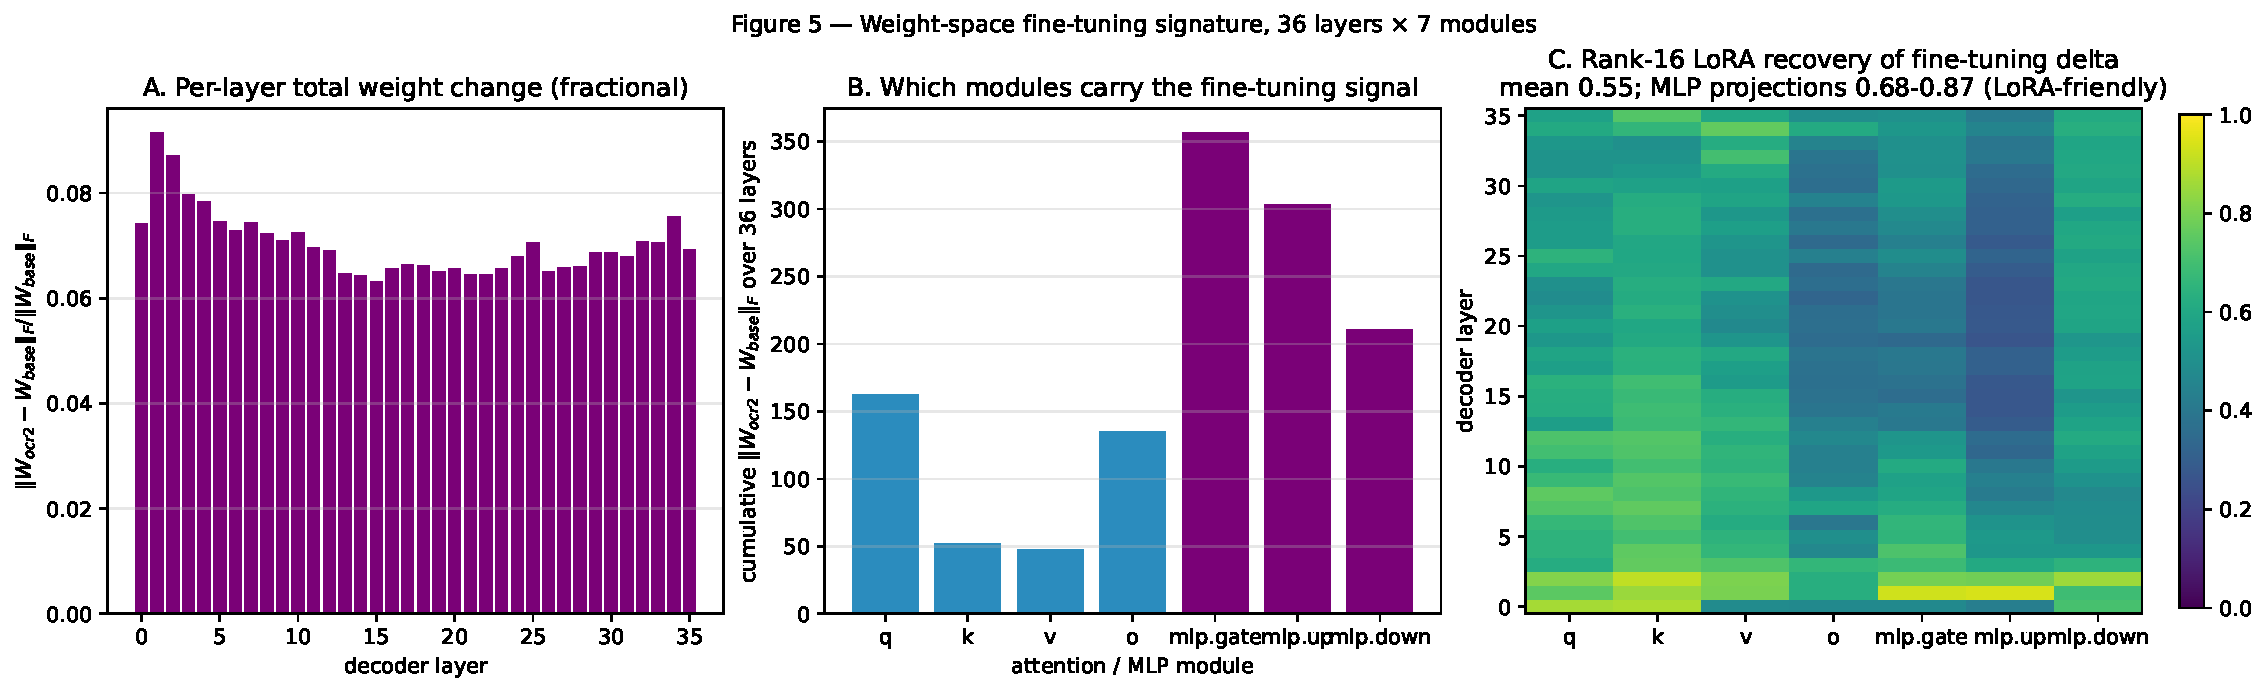
\includegraphics[width=\linewidth]{fig5_weight_diff.pdf}
\caption{Per-module cumulative Frobenius weight diff between OCR2 and base, summed across 36 decoder layers. The three MLP projections (\texttt{gate\_proj}, \texttt{up\_proj}, \texttt{down\_proj}) together account for 69\% of the total change. Fractional change per layer (diff norm / base norm) is near-uniform at 0.06--0.09 across the 36 layers --- the weight edit is not concentrated in any specific layer.}
\label{fig:weight}
\end{figure}

Residual-stream and attention-pattern analyses measure \emph{effects}. Figure~\ref{fig:weight} measures the cause directly: per-module Frobenius diff between OCR2 and base weights, summed over layers.

\begin{itemize}[leftmargin=1.4em,itemsep=0pt,topsep=2pt]
\item \texttt{mlp.gate\_proj}: 356 (28\% of total).
\item \texttt{mlp.up\_proj}: 304.
\item \texttt{mlp.down\_proj}: 211.
\item \texttt{q\_proj}: 163. \quad \texttt{o\_proj}: 135.
\item \texttt{k\_proj}: 52. \quad \texttt{v\_proj}: 48.
\end{itemize}

MLPs total 871 of the 1268 total change, i.e.\ 69\%. Attention projections account for 31\%, and within attention, query and output projections dominate; keys and values barely move. This is consistent with a fine-tune that rewires how information is computed inside each layer's FFN, and how outputs are formed from attention reads, rather than what keys are compared against.

Unlike the residual-stream signal, the weight edit is not layer-concentrated. Per-layer fractional change (diff norm / base norm) sits at 0.06--0.09 across all 36 decoder layers, with the maximum at L1 (0.092). The fine-tune touched every layer; the residual-stream effects concentrate in the upper decoder because deltas compound during the forward pass, not because the upper decoder's weights moved more.

Rank-truncated SVDs of the per-module diff give a more nuanced picture than the cumulative-Frobenius bar chart alone suggests. Rank-16 recovery (mean across the 36 layers) is highest for the attention K, Q, V projections (0.67, 0.62, 0.61) and lowest for \texttt{mlp.up\_proj} (0.39) and \texttt{o\_proj} (0.44); \texttt{mlp.gate\_proj} sits at 0.52 and \texttt{mlp.down\_proj} at 0.59. Rank-16 captures the MLP signal less cleanly than it captures the attention signal, even though the MLPs carry a larger cumulative Frobenius share (69\% vs.\ 31\%). The two properties pull in opposite directions. A team adapting a Qwen2.5-VL-3B-scale model to a new OCR domain can resolve this practically: since MLPs carry the bulk of the fine-tune's weight signature, a rank-16 LoRA on \texttt{mlp.gate\_proj} and \texttt{mlp.up\_proj} across all 36 layers captures the largest share of the actual edit that Nanonets made, but full-fidelity reproduction would require either higher rank on MLPs or combining MLP LoRA with a lower-rank LoRA on Q/K/V. At rank 16 alone, MLP coverage is the better compute-per-signal trade than any attention-module placement at this checkpoint scale.

\subsection{The vision encoder moves in OCR2 but not in OCR-s: the ViT edit is fine-tune-specific}
\label{sec:vit}

\begin{figure}[t]
\centering
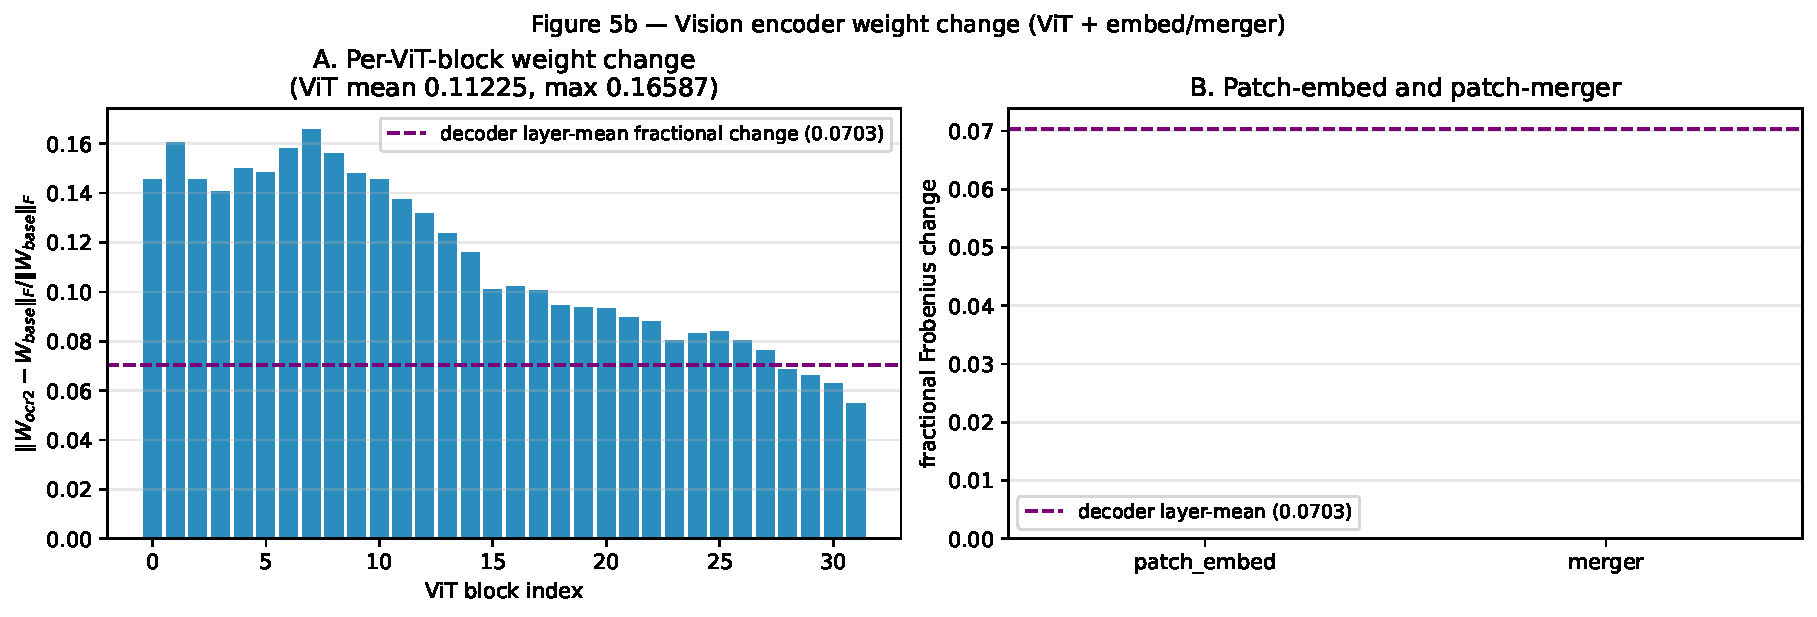
\includegraphics[width=\linewidth]{fig5b_vit_weight_diff.pdf}
\caption{Per-block fractional Frobenius weight diff (diff norm / base norm) between OCR2 and base, inside the ViT vision tower. Mean across the 32 transformer blocks is 0.112, with an early-to-late gradient from $\sim 0.15$ at block 0 to $\sim 0.05$ at block 31 and a peak of 0.166 at block 7. For comparison, the decoder's mean per-layer fractional change is 0.070 --- OCR2's ViT is $1.60\times$ more perturbed per-layer than its decoder. Patch-embed and patch-merger modules are near-zero change ($< 0.01$).}
\label{fig:vit}
\end{figure}

\begin{figure}[t]
\centering
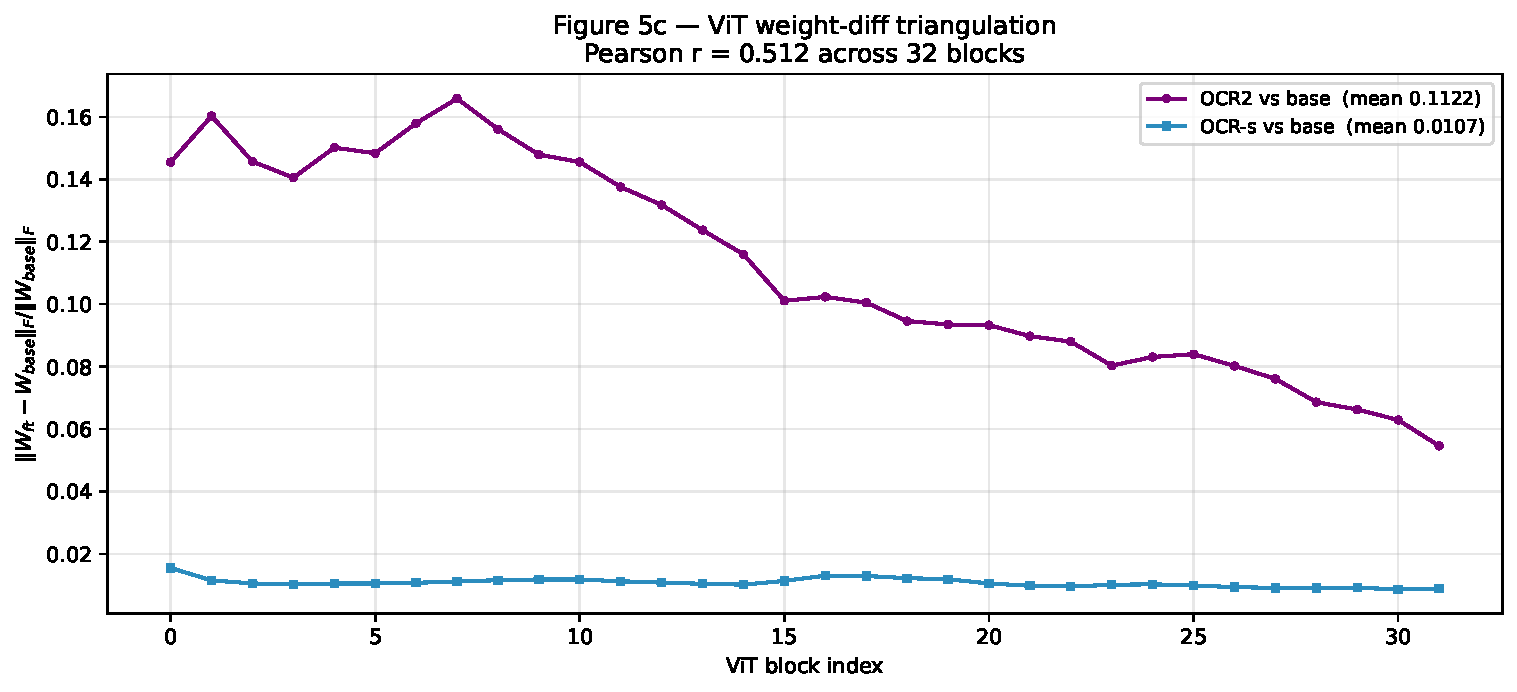
\includegraphics[width=\linewidth]{fig5c_vit_weight_diff_triangulation.pdf}
\caption{ViT weight diff for both fine-tunes against base. OCR-s's mean per-block fractional change is 0.011, an order of magnitude less than OCR2's 0.112 and less than the decoder's 0.070. The two per-block curves correlate at Pearson $r = 0.51$, compared to $r = 0.996$ on the decoder's 37-layer residual curves. The ViT perturbation is not a general property of OCR fine-tuning the Qwen2.5-VL-3B-Instruct base; it is specific to Nanonets-OCR2-3B's training.}
\label{fig:vit-triangulation}
\end{figure}

A direct OCR2-vs-base weight diff on the vision tower shows mean per-block fractional change of 0.112 against 0.070 in the decoder --- OCR2's vision encoder is perturbed $1.60\times$ more per layer than its decoder (Figure~\ref{fig:vit}). The change has an early-to-late gradient: early ViT blocks move most ($\sim 0.15$ at block 0), the peak sits at block 7 (0.166), and late blocks taper to $\sim 0.05$ at block 31. The pixel-side patch embedding and the patch-merger projection onto the LLM hidden space are near-zero (both $< 0.01$). Only the ViT transformer stack itself moved, and it moved disproportionately for this fine-tune.

The symmetric measurement on OCR-s reframes the result (Figure~\ref{fig:vit-triangulation}). OCR-s's mean per-block fractional ViT change is $0.011$ --- an order of magnitude smaller than OCR2's and \emph{less} than OCR-s's own decoder-layer mean. Across the 32 ViT blocks, OCR2 and OCR-s correlate at Pearson $r = 0.51$, against $r = 0.996$ on the decoder's 37-layer residual curves. Two fine-tunes of the same base on overlapping OCR objectives can make very different choices about how much the vision encoder moves during training. The ViT edit is a training-recipe property of OCR2 specifically, not of OCR fine-tuning the shared base writ large.

This actually strengthens the decoder-side triangulation. The decoder pattern ($r = 0.996$) is evidence the residual-stream localization is a structural property of the base, reproducible across fine-tunes. The ViT pattern is not such evidence --- the two fine-tunes diverge there. For a downstream team, the practical implication is: \emph{the decision to move the ViT during an OCR fine-tune is a training-time hyperparameter choice}, not a structural requirement of the task. OCR-s reached a competitive task quality on typewritten documents (per its public release notes) with a near-frozen ViT. An adaptation workflow can start with a frozen ViT by default, and unfreeze selectively if a specific content vertical needs visual-stream specialization.

\subsection{Head-level patching at L11: destabilization gradient, but no OCR-directional flip}
\label{sec:head-patching}

\begin{figure}[t]
\centering
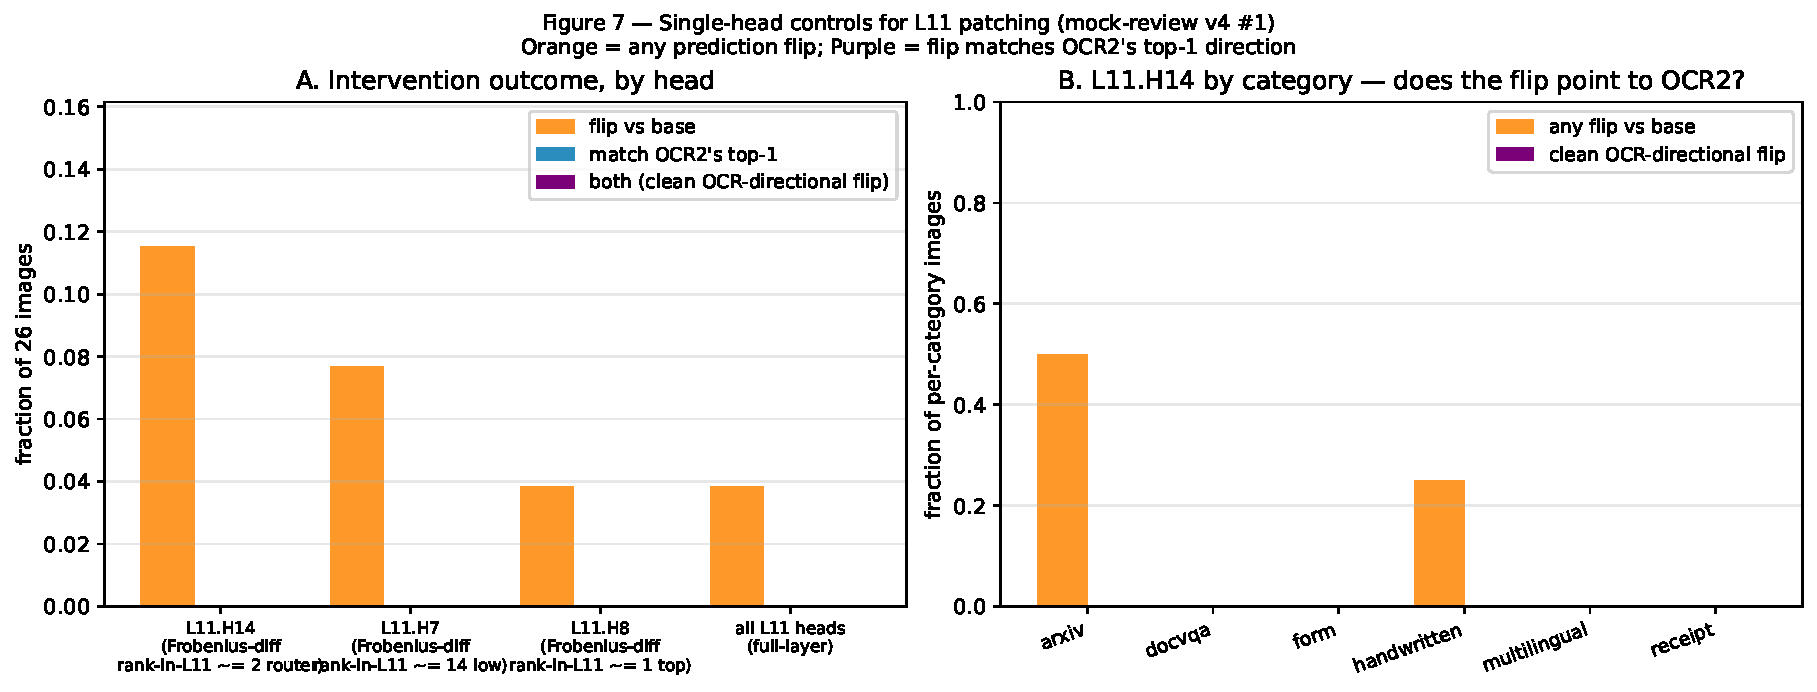
\includegraphics[width=\linewidth]{fig7_single_head_controls.pdf}
\caption{Head-level patching at L11 with three single-head interventions and a full-layer control, $N = 26$ images. For each image we capture OCR2's L11 pre-$W_o$ attention output, replace one of \{H14 router (Hua et al.), H7 low-Frobenius control, H8 highest-Frobenius-at-L11\}, or all 16 heads, and let base continue forward. Panel A: orange = flip vs.\ base; blue = match OCR2's own top-1; purple = both (OCR-directional flip). Blue and purple are 0 for every intervention --- no single-head patch and no full-layer patch redirects base's prediction toward OCR2's. H14 destabilizes 3/26; H7 destabilizes 2/26; H8 destabilizes 1/26; full-layer 1/26. Panel B breaks out H14 by category: the 3 destabilized images are 2 arXiv-equation and 1 handwritten; zero flips on docvqa, forms, receipts, multilingual.}
\label{fig:head-patch}
\end{figure}

\S\ref{sec:router-stable} leaves open whether L11.H14's stable attention pattern implies it is peripheral, or whether its routing function is preserved across fine-tuning while its output is used differently downstream. We test this directly by capturing OCR2's L11 per-head attention output via \texttt{forward\_pre\_hook} on \texttt{o\_proj} (pre-projection shape $[T, 16, 128]$) and patching selected head slices into base's forward. Three head targets: H14 (the Hua router, rank-141-of-576), H7 (low Frobenius diff within L11, $\delta = 3.82$, an explicit random control), H8 (highest Frobenius diff within L11, $\delta = 6.20$). We also patch all 16 heads as the full-layer comparison. For each intervention we record base's top-1, OCR2's own top-1 at the same position, and the patched top-1.

The headline result is that \emph{no patch at all moves base toward OCR2}. OCR2 and base disagree on the top-1 for all 26 images (base typically predicts modality-boundary tokens like \texttt{<img>}, OCR2 predicts content-specific tokens), and the patched base never matches OCR2's top-1 under any single-head or full-layer intervention. The flips reported earlier in our infrastructure (flip $\equiv$ patched top-1 $\neq$ base top-1) all land in a small token set \{27, 73594, 8420, 785\}; base's own preferred top-1's across the 26 images are \{27, 73594, 8420\} and token 785 appears only as a patched output (image 14 under H14), so these flips are destabilizations within a narrow-vocabulary neighborhood, not OCR-directional interventions.

That leaves the flip-rate gradient as the informative signal. H14 destabilizes 3/26 predictions, H7 2/26, H8 1/26, and the full-layer swap 1/26. H14's destabilization footprint is not maximal within L11 (H7 destabilizes image 09 and image 11, H8 destabilizes image 09, overlapping with H14's targets), but H14 has the broadest footprint, and single-head patching destabilizes more than full-layer patching --- the three destabilized images are specifically arXiv-equation and handwritten content, the same categories that cluster at the L0--L2 residual threshold in \S\ref{sec:causal}. Attention-pattern rank within L11 is only weakly predictive: H8 outranks H14 by Frobenius diff but H14 destabilizes more, and H7 (rank 14 of 16 within L11) destabilizes more than H8 (rank 1 within L11).

The mechanistic implication is subtler than v3's L11.H14-specific story suggested. The mid-cluster residual-level threshold at L9--L15 (\S\ref{sec:causal}) is not reproduced by any single L11 attention head or by the full L11 attention layer. It must be driven by L11's MLP, Q/V projections under a full residual-stream swap, cross-layer dynamics between L11 and L12+, or some combination --- components that a pre-$W_o$ attention intervention cannot reach. The residual-stream intervention in \S\ref{sec:causal} replaces the entire state at layer $L$, which is a broader change than swapping only $W_o$'s input, and only the broader intervention flips top-1 predictions in a way that matches (or at least is consistent with) OCR2's behavior. L11.H14 carries a modest, category-biased destabilization signal but is not the mechanistic pivot the original L11-threshold reading suggested. Head-level interchange interventions \citep{vig2020causal, geiger2021interchange} on the full per-head attention output cannot substitute for full residual-stream patching in this kind of VLM.

\subsection{Reverse-direction patching: base residuals destabilize OCR2 but never match it}
\label{sec:reverse-patching}

\begin{figure}[t]
\centering
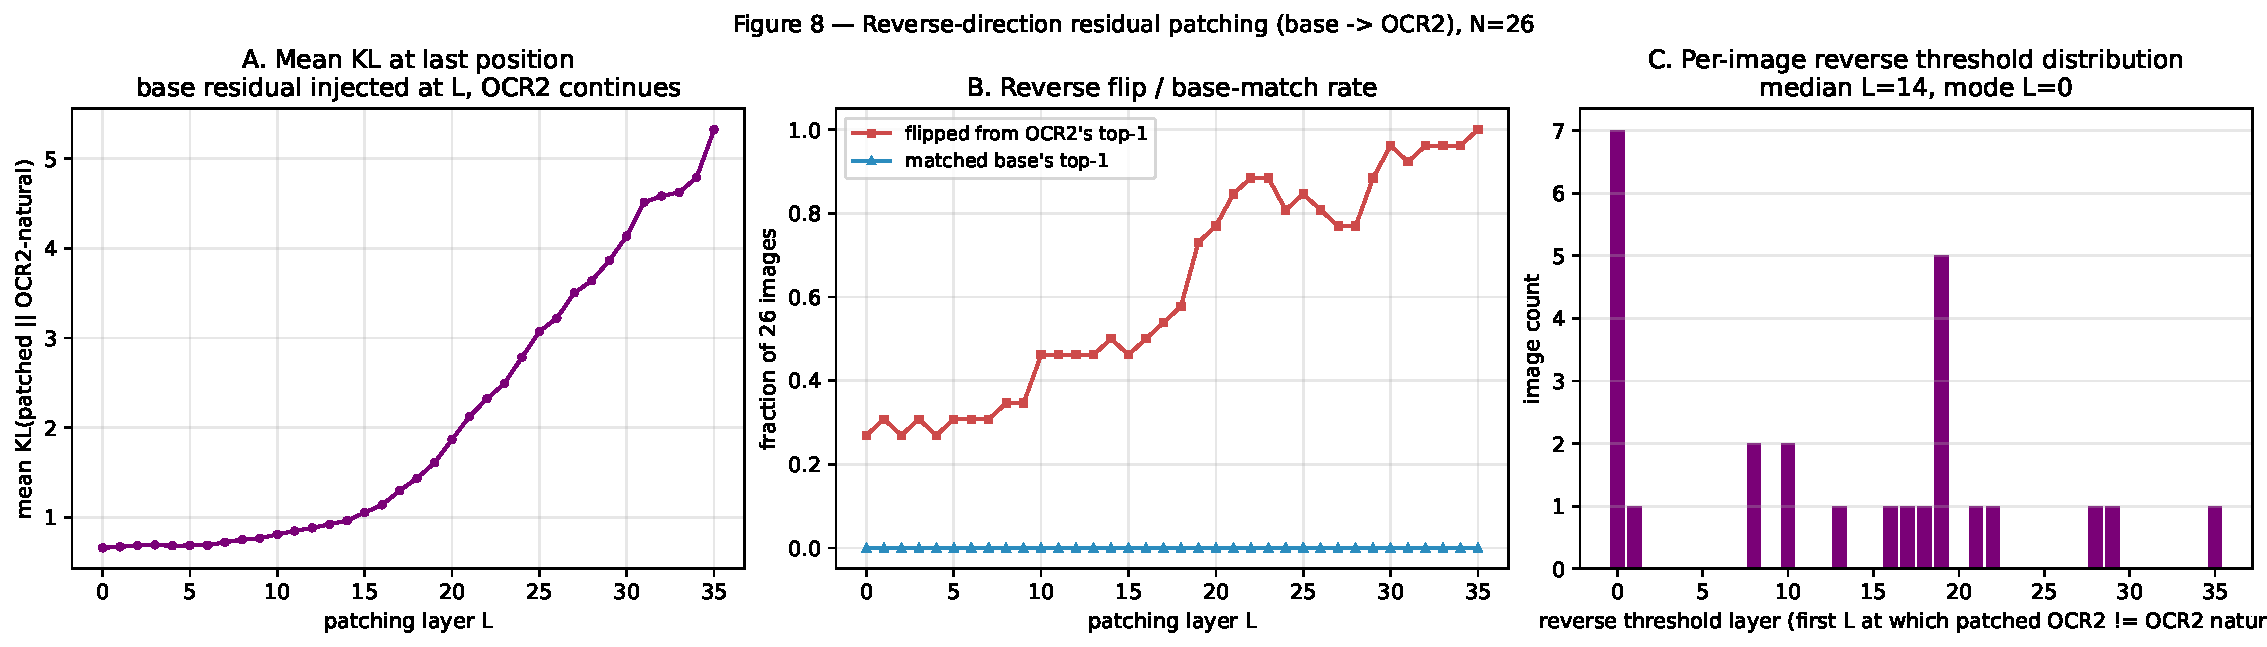
\includegraphics[width=\linewidth]{fig8_reverse_patching.pdf}
\caption{Reverse-direction residual patching: base's cached residual state at layer $L+1$ is injected into OCR2's forward at layer $L$, for each of the 26 images and each of 36 decoder layers. Panel A: mean KL between the patched OCR2 and OCR2's natural distribution at the last-token position. Panel B: fraction of images whose patched top-1 (i) flips away from OCR2's natural top-1 (red) and (ii) matches base's natural top-1 (blue). The blue line is zero at every layer: 0/26 patched OCR2 predictions ever match base's prediction. Panel C: per-image reverse-threshold distribution (first $L$ at which patched OCR2 top-1 $\neq$ OCR2 natural top-1). Median $L = 14$, mode $L = 0$ (7 images), mean $L = 12.7$.}
\label{fig:reverse-patching}
\end{figure}

The forward direction in \S\ref{sec:causal} shows OCR2's residual state at layer $L$ is sufficient to flip base's top-1 at per-image threshold layers. The symmetric question --- would base's residual state break OCR2's prediction at the same layers --- sets up a test for whether the causal story is bidirectional, and whether injecting base residuals ever redirects OCR2 toward base's prediction.

We load OCR2 once and patch each decoder layer's output with base's cached $h_{L+1}$ from the Phase 2.2 cache. Figure~\ref{fig:reverse-patching} (Panel B) shows the outcome. Reverse flips (patched OCR2 $\neq$ OCR2 natural) do happen and rise with depth, reaching 100\% by L22. But the blue line --- patched OCR2 $=$ base natural top-1 --- is flat at zero. Zero of 26 images ever produce base's top-1 at any layer, under any patching depth. The reverse intervention destabilizes OCR2's prediction but does not redirect it toward base's.

The per-image threshold distribution (Panel C) is not bimodal like the forward direction. It spreads from $L = 0$ (7 images, where even injecting base's embedding flips OCR2) through $L = 35$ (1 image, where only the last layer patching breaks OCR2). Median $L = 14$, mean $L = 12.7$. Seven of the 26 images are fragile enough that base's embedding alone breaks OCR2's forward; seven others have thresholds $19 \leq L \leq 27$; three images require $L \geq 28$ to flip.

The mechanistic reading: OCR2's forward pass is built around OCR2-specific residual representations, and injecting base's state destabilizes the pipeline without redirecting it toward base's output. A subtlety worth naming: because OCR2's own \texttt{lm\_head} is random (\S\ref{sec:method}), both OCR2's natural prediction and the reverse-patched prediction are evaluated via base's tied unembedding. The asymmetry is therefore between two projections \emph{in the same basis}: (patched OCR2) $\to$ base-unembed vs.\ (natural OCR2) $\to$ base-unembed. The result is that OCR2's upper-decoder transforms base's injected residual into a configuration whose base-unembed projection is neither OCR2's own corrected prediction nor base's. The reverse direction does not redirect in either basis. The asymmetry between this reverse direction and the forward direction \S\ref{sec:causal} is consistent with fine-tuning as a \emph{specialization} of the base's decoder geometry. In the forward direction, base accepts OCR2's residual as a substrate and its remaining layers carry the OCR2-patched state to an OCR2-consistent prediction at mid-to-late layers (the shared lm\_head over OCR2's upper-decoder state projects directly to OCR2's own top-1 at late $L$). In the reverse direction, OCR2 does not accept base's residual as a substrate: its remaining layers transform base's residual into a configuration that produces neither OCR2's nor base's prediction.

\subsection{Random-residual control: the match rate is fine-tune-specific}
\label{sec:random-control}

\begin{figure}[t]
\centering
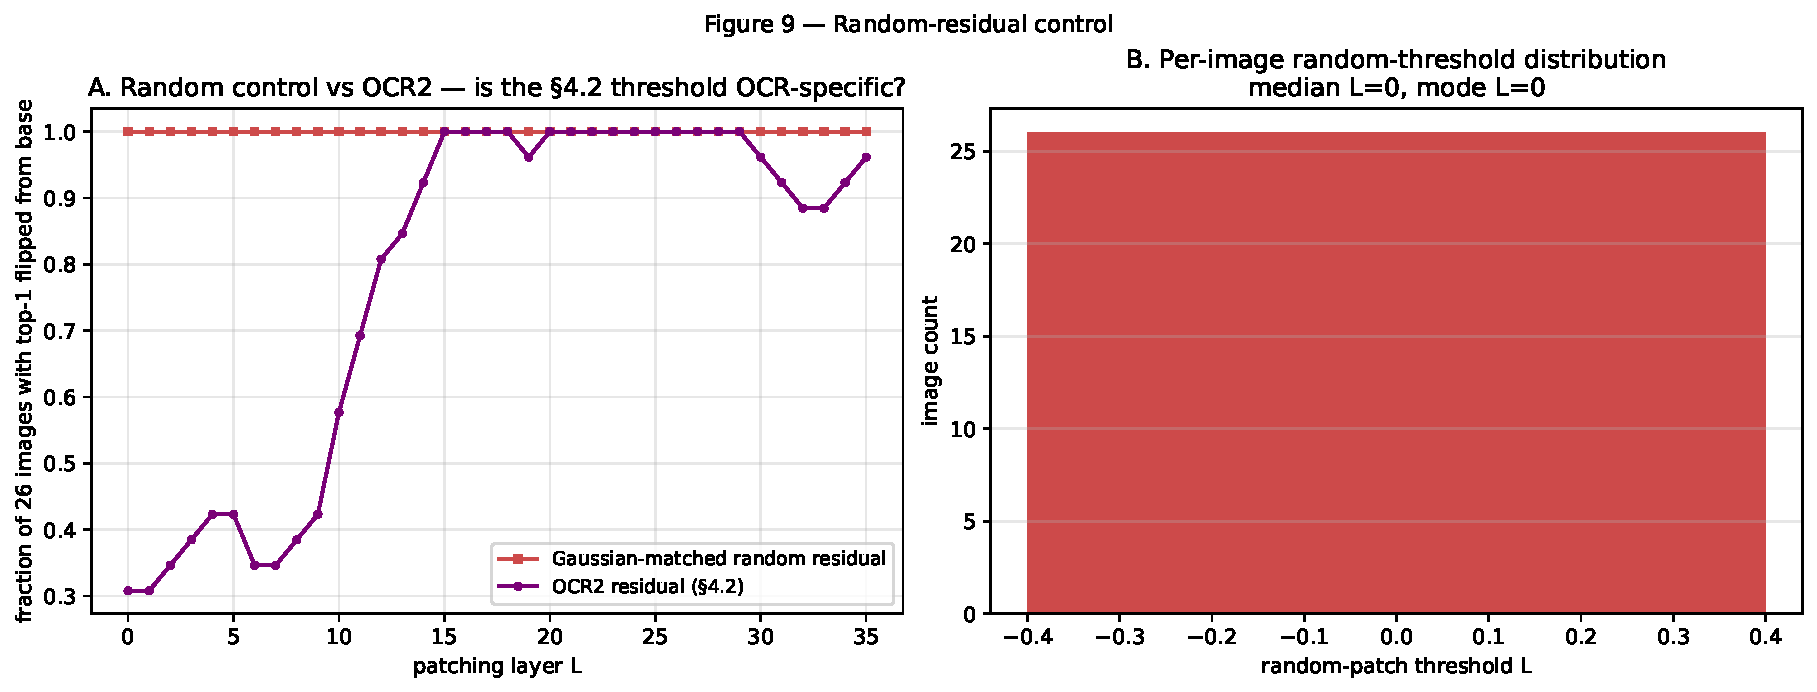
\includegraphics[width=\linewidth]{fig9_random_control.pdf}
\caption{Random-residual control: for each image and each layer $L$, a Gaussian tensor matched to OCR2's per-token L2 norm at layer $L$ is injected into base's forward at decoder layer $L$, in place of OCR2's cached residual. Left panel: random flip rate (magenta) against OCR2 flip rate (purple). Both reach 100\% at or near L0. Right panel: per-image random threshold distribution; median $L = 0$, mean $L = 0$. A seeded match-OCR2-corrected audit (post-hoc on the stored patched top-1's) gives the numbers in the body text.}
\label{fig:random-control}
\end{figure}

The flip-rate curve in Figure~\ref{fig:patching} and the match rate in Figure~\ref{fig:fwd-match} establish that OCR2's residuals are causally sufficient at the per-image threshold. But the mock reviewer raised a legitimate question the forward patching alone cannot settle: is the match rate a fine-tune-specific property of OCR2's residual, or would \emph{any} residual of matched magnitude flip the prediction the same way? We test this with a random-residual control. For each image $x$ and each decoder layer $L$, we draw $r \sim \mathcal{N}(0, I)$ of the same shape as OCR2's cached $h_L(x)$, rescale $r$ so its per-token L2 norm matches OCR2's per-token norm at that layer, and patch base's forward with $r$ at layer $L$. The seed is fixed for reproducibility.

Flip-vs-base rates under the random control reach 100\% at L0 and stay there (Figure~\ref{fig:random-control}): matched-magnitude noise at the input destabilizes every image, every layer. That is the weak sense in which ``any sufficiently-perturbed residual flips the prediction.'' But the match-vs-OCR2-corrected rates are flat at zero for almost every layer, peaking at 3.85\% (1/26 images) at L14. Twenty-five of 26 images never produce OCR2's corrected top-1 at any layer under a random patch; across all 936 layer-image patching trials, only a single image produces any OCR-directional matches --- 2 of its 36 layer-trials land on OCR2's corrected top-1 (L14 and L34 for image 21), which is well below chance for a 151,936-token vocabulary and consistent with coincidence. Structured OCR2 residuals match OCR2 at 92.3\% peak; random matched-magnitude residuals match at 3.85\% peak. The factor-of-24 differential is the cleanest confirmation that the \S\ref{sec:causal} causal signal is content-specific to the fine-tune's residual-space configuration rather than generic perturbation-tolerance of the base's downstream layers.

\section{Discussion}
\label{sec:discussion}

\paragraph{From correlational to causal, and the causal story is task-conditional.} The residual-stream peak at L35 and the bimodal attention split are correlational. The activation-patching results are causal: replacing the base's residual stream with OCR2's at the per-image threshold layer is \emph{sufficient} to flip the top-1. But the threshold is not a single layer. It is bimodal, and the mode --- input-layers versus mid-decoder --- is determined by whether the base can already read the content. This suggests a generalization for how to think about SFT localization: the right question is not ``which layer does this fine-tune act at,'' but ``which stage of the base's own pipeline does the fine-tune override, given what the base already does with this input.'' Content inside the base's repertoire gets overridden late; content outside it gets re-encoded from the beginning. Two pipeline stages, one fine-tune.

\paragraph{Head-level patching is not sufficient for OCR-directional redirection.} A head-level patching sweep at L11 (\S\ref{sec:head-patching}) turns out to be a cleaner probe than the original L11.H14 check \S\ref{sec:router-stable} framed. The direct observation is that zero of four interventions --- H14-only, H7-only (low-Frobenius control), H8-only (highest-Frobenius control within L11), and the full-layer swap --- ever produce base predictions that match OCR2's. Residual-stream patching in \S\ref{sec:causal} does produce OCR-directional flips at specific per-image thresholds; the head-level intervention does not. The residual-stream swap replaces the entire $h_L$ at layer $L$, whereas swapping the pre-$W_o$ head output replaces only one head's contribution. The gap between those two --- the residual state reproduces OCR2, the single-head attention does not --- tells us the causal work at the mid-cluster threshold lives in the L11 MLP or in cross-layer interactions between L11 and $L > 11$ that a pre-$W_o$ attention hook does not reach. L11.H14 is not the mechanistic pivot the original L11-threshold reading suggested; it is a modestly-destabilizing head whose attention pattern happens to remain stable under fine-tuning.

\paragraph{Implications for differential adaptation.} The results suggest a few operational moves for anyone studying or performing an OCR-style fine-tune on a similar VLM. First, the weight-diff signature is a concrete LoRA starting point. MLPs carry 69\% of the Frobenius change, and rank-16 SVD recovers 0.39--0.59 of each MLP module's energy --- so a rank-16 LoRA on \texttt{mlp.gate\_proj}, \texttt{mlp.up\_proj}, and \texttt{mlp.down\_proj} captures roughly 24--34\% of the total fine-tune edit. Rank-16 recovery is cleaner on attention Q/K/V (0.61--0.67), so a full-recipe adaptation would pair MLP placement with lower-rank Q/K/V coverage. The operational move is that MLPs are where to spend the rank budget, not that rank-16 alone is sufficient. Second, the bimodal-threshold result has a direct placement implication: content outside the base's reading repertoire (handwriting, non-Latin scripts, structured symbols) needs input-layer LoRAs (L0--L2) in addition to mid-decoder ones, because the causal edit lives at the input for that kind of content. Content the base already reads can be adapted at mid-decoder alone. Third, for layer-wise learning-rate scheduling, the NAST framework \citep{sim2026layerspecific} uses causal-tracing effect scores to scale per-layer gradient updates; the per-image patching curves (Figure~\ref{fig:patching}) are a direct analogue, with the refinement that the scheduler should be content-aware rather than uniform.

\paragraph{Cross-scale transfer.} \citet{tigges2024circuitscale} show on 70M--2.8B Pythia that circuit-level algorithms are stable across scale over 300B training tokens, even as the specific head indices implementing them drift. That pattern would predict that whatever algorithmic signature OCR fine-tuning leaves in a 3B dense model --- upper-decoder residual-stream accumulation, MLP-heavy weight movement, stable cross-modal arbitration --- should have structural analogues in a 35B MoE, even if the exact head and layer indices look different. This is a transferability hypothesis, not a guarantee.

\paragraph{What surprised us.} The vision encoder was not where we expected the fine-tuning payload to live, and on OCR2 it turned out to be substantially perturbed ($1.60\times$ the decoder's per-layer fractional change, with an early-block gradient). The symmetric measurement on OCR-s then surprised us a second time: its ViT fractional change is only $0.011$, an order of magnitude smaller than OCR2's and smaller than the decoder's own mean. The choice to move the ViT heavily is a Nanonets training decision specific to OCR2, not a consequence of OCR fine-tuning the shared base. Whether OCR2's higher ViT perturbation corresponds to a functional advantage on any specific document category is a separate question --- head-level attention-pattern diffs on the ViT for both fine-tunes are the cleanest next step.

\paragraph{What we don't have.} Single-seed activation patching on 26 images, no head-level patching sweep, no ablation studies. No attention-pattern diff on the ViT (only a weight diff), and no ViT-side measurement on OCR-s --- so the triangulation argument for the decoder localization does not extend to the vision tower. No modality-probe evidence for Claim 3 --- the probe was position-trivial and pivoted to a ceiling-effect null. Per-category $n$ on the bimodal threshold split is 4--6 images, enough to separate the two clusters but not to finely rank within them. Every one of these gaps is a natural follow-up and is enumerated in \S\ref{sec:conclusion}.

\section{Conclusion}
\label{sec:conclusion}

Four complementary diagnostics --- residual-stream diffs, attention-pattern diffs, residual- and head-level activation patching, and per-module weight diffs --- applied to Nanonets-OCR2-3B and its Qwen2.5-VL-3B-Instruct base converge on a specific picture. The representational edit concentrates in the upper decoder and peaks at L35 with Pearson $r = 0.996$ between two independently-trained fine-tunes, and the L35 peak is text-dominated (53\% pre-image instruction, 27\% post-image, 20\% image tokens). The layer at which patching OCR2's residual into the base is causally sufficient to flip the top-1 is bimodal across documents: layers 0--2 for handwriting, LaTeX equations, and non-Latin scripts (11/26 images); layers 9--15 for English typewritten documents, forms, and receipts (15/26 images). The Hua et al.\ router head L11.H14 sits at rank 141 of 576 in the attention-pattern diff. Head-level patching at L11 --- H14, two single-head controls, and the full attention layer --- never redirects base toward OCR2's top-1; the largest effect is a 3/26 destabilization under H14-only, consistent with a modest category-biased role (flips 2/4 arXiv + 1/4 handwritten). The mid-decoder residual-level threshold at L9--L15 is not reproduced by any attention-only intervention and must therefore involve L11's MLP or cross-layer dynamics. Among the top-12 high-Frobenius heads, the L0 cluster re-encodes the visual input and the L30--33 cluster increases attention to structured markers, with 11/12 marker-diff CIs excluding zero. In parameter space, 69\% of the Frobenius change is concentrated in the three MLP projections, with gate and up projections carrying most of that; per-block activation contribution concentrates at the last six decoder blocks (L30--L35 = 46.3\%) even though the weight change is nearly uniform. OCR2's vision encoder is perturbed 1.60$\times$ more per layer than its decoder (mean fractional change 0.112 vs.\ 0.070) with a gradient from $\sim$0.15 at block 0 to $\sim$0.05 at block 31, but OCR-s's ViT moved only 0.011 on the same axis. The two fine-tunes correlate at Pearson $r = 0.51$ on ViT curves against $r = 0.996$ on decoder residual curves --- the ViT edit is OCR2-specific, not general.

The natural follow-ups are the symmetric ablation direction (zero-out top-12 heads in OCR2 and measure degradation on structured-marker emission); a head-level patching sweep across all 576 heads to identify other mechanistically-active heads beyond L11.H14; larger per-category $n$ to refine the bimodal-threshold split within the early and middle clusters; a content-conditional probe for structured-output mode that is not defeated by positional trivialities; and a symmetric vision-encoder measurement on OCR-s plus a head-level ViT attention-pattern diff, now that the decoder-only assumption has been ruled out (\S\ref{sec:vit}). For a team producing the next generation of an OCR-specialized VLM, the findings here are a diff-based baseline map of what a structurally similar fine-tune moves --- which is a different kind of answer than ``where does OCR live'' in a trained model, and complementary to it.

\paragraph{Research harness.} Theoria (author's own tooling). Experiments and writing were produced within a single autonomous run; manual author review followed.

\bibliographystyle{plainnat}
\bibliography{references}

\end{document}
